\section{Grafi}

Un grafo \`e una coppia $(V,E)$ di vertici e archi (edges). I vertici sono dei punti (o nodi), e gli archi (o lati) sono un insieme di coppie di vertici $\{u, v\}$, con $u, v \in V$.

Gli archi possono essere diretti (o orientati). In questo caso $(u,v)$ con $u,v \in V$ \`e un arco diretto da $u$ a $v$. Non necessariamente c'\`e anche un arco da $v$ a $u$.

Se gli archi sono diretti, si parla di grafo diretto, altrimenti di grafo indiretto o semplicemente di grafo.

Dato un arco $\{u,v\}$ si dice che l'arco \`e incidente ai vertici $u$ e $v$, e che i vertici $u$ e $v$ sono adiacenti.

Il numero di archi incidenti con un dato vertice $v$ \`e detto grado del vertice $v$, e si indica con $\deg (v)$.

L'esempio tipico di problema risolvibile con i grafi \`e quello dei ponti della citt\`a di K\"{o}nigsberg. 

\begin{figure}
\centering
\caption{Rappresentazione schematica della citt\`a di K\"{o}nigsberg: gli archi sono i ponti}
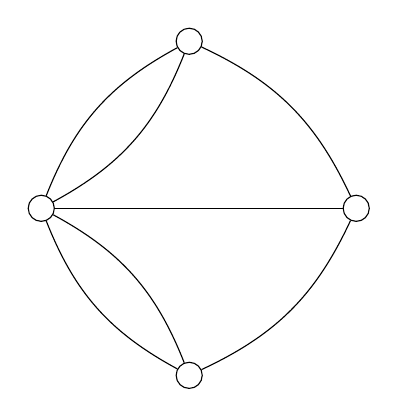
\begin{tikzpicture}[node distance = 3cm]
    \node (E) [circle, draw] {};
    \node (N) [above left of=E, circle, draw] {};
    \node (S) [below left of=E, circle, draw] {};
    \node (W) [left of=E, node distance=4cm, circle, draw] {};

    \path [-] (E) edge [bend right=20] (N)
              (E) edge [bend left=20] (S)
              (E) edge (W)
              (W) edge [bend left = 20] (N)
              (W) edge [bend right = 20] (N)
              (W) edge [bend left = 20] (S)
              (W) edge [bend right = 20] (S);
\end{tikzpicture}
\end{figure}

La domanda \`e: dato un grafo, esiste un cammino che attraverso ogni arco esattamente una volta? Un cammino in un grafo \`e una serie di vertici e archi, $v_0 e_1 v_1 e_2 x_2 \dots$, dove $e_i$ \`e l'arco che collega i vertici $x_{i - 1}$ e $x_{i}$.

Il problema del cammino per K\"{o}nigsberg \`e che alcuni vertici hanno un grado dispari.

\begin{defn}[Cammino Euleriano]
Un cammino euleriano \`e un cammino che inizia e finisce dallo stesso vertice e usa ogni arco esattamente una volta.
\end{defn}

Quel che abbiamo appena osservato \`e che se un grafo ha un nodo v con grado dispari, non esiste un cammino Euleriano. Quindi condizione necessaria affinch\'e esista un cammino Euleriano \`e che il grafo abbia tutti vertici con grado pari. \`E anche condizione sufficiente? No, il grafo deve anche essere \emph{connesso}. Le due condizioni, assieme, sono sufficienti.

\begin{figure}
\centering
\caption{Grafo non connesso, ma in cui ogni nodo ha grado pari}
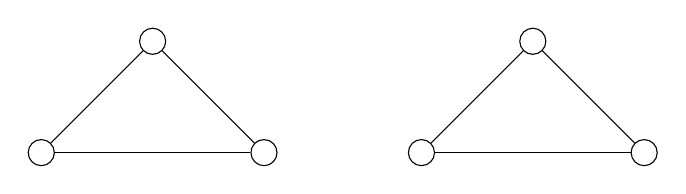
\begin{tikzpicture}[node distance=2cm]
    \node (1) [circle, draw] {};
    \node (2) [circle, draw, below left of=1] {};
    \node (3) [circle, draw, below right of=1] {};
    \node (4) [circle, draw, right of=3] {};
    \node (5) [circle, draw, above right of=4] {};
    \node (6) [circle, draw, below right of=5] {};

    \path[-] (1) edge (2)
             (2) edge (3)
             (1) edge (3)
             (4) edge (5)
             (4) edge (6)
             (5) edge (6);
\end{tikzpicture}
\end{figure}

\begin{theorem}
Sia $G$ un grafo connesso, $G$ contiene un cammino Euleriano $\iff$ ogni vertice ha grado pari. Esiste inoltre un algoritmo per trovare tale cammino.
\end{theorem}

Ci sono due aspetti da approfondire: il concetto di ``connessione'', e gli algoritmi sui grafi.

Partiamo dagli algoritmi: bisogna chiedersi prima di tutto come viene rappresentato il grafo per il computer. Ci sono principalmente due modi per rappresentarlo:
\begin{description}
    \item[Matrice di adiacenza] La matrice di adiacenza $M$ ha $n$ righe e $n$ colonne, con $\abs{V} = n$. $m_{i,j}$ \`e 1 se $v_i \adj v_j$ (i vertici $v_i$ e $v_j$ sono adiacenti), 0 se non sono adiacenti.
    \begin{figure}[h]
    \centering
    \caption{\label{fig:matrice_grafo_indiretto}Grafo indiretto}
    \begin{tikzpicture}[node distance=3cm]
        \node (1) [circle, draw] {1};
        \node (2) [circle, draw, below left of=1] {2};
        \node (4) [circle, draw, below right of=1] {4};
        \node (3) [circle, draw, below right of=2] {3};

        \path [-] (1) edge (2)
                  (1) edge (3)
                  (1) edge (4)
                  (2) edge (3)
                  (3) edge (4);
    \end{tikzpicture}
    \end{figure}
    \[
    \begin{pmatrix}
    0 & 1 & 1 & 1 \\
    1 & 0 & 1 & 0 \\
    1 & 1 & 0 & 1 \\
    1 & 0 & 1 & 0
    \end{pmatrix}
    \]
    In questo caso il grafo non \`e diretto, ed \`e quello in figura \ref{fig:matrice_grafo_indiretto}. Se invece il grafo \`e diretto, come quello in figura \ref{fig:matrice_grafo_diretto}:
    \begin{figure}[h]
    \centering
    \caption{\label{fig:matrice_grafo_diretto}Grafo diretto}
    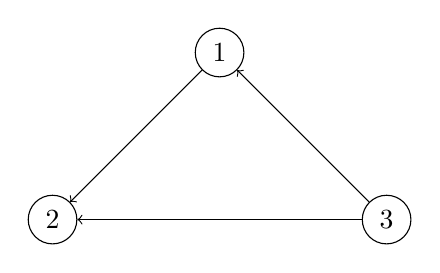
\begin{tikzpicture}[node distance=3cm]
        \node (1) [circle, draw] {1};
        \node (2) [circle, draw, below left of=1] {2};
        \node (3) [circle, draw, below right of=1] {3};

        \path [->] (1) edge (2)
                   (3) edge (1)
                   (3) edge (2);
    \end{tikzpicture}
    \end{figure}
    \[
    \begin{pmatrix}
    0 & 0 & 1 \\
    1 & 0 & 1 \\
    0 & 0 & 0
    \end{pmatrix}
    \]
    Lo spazio occupato \`e $O(n^2)$. Per vedere se due vertici $v_i$ e $v_j$ sono adiacenti, il tempo \`e costante ($O(1)$). Ma grafi con certe caratteristiche sprecare dello spazio, che si pu\`o risparmiare sapendo in partenza che il grafo ha meno archi di $n^2$.
    \item[Lista delle adiacenze] Ho una lista dei vertici, e a ogni vertice associo una lista delle adiacenze. La lista di adiacenze del grafo in figura \ref{fig:matrice_grafo_indiretto} \`e:
    \begin{align*}
    v_1 &\to [2, 3, 4] \\
    v_2 &\to [1, 3] \\
    v_3 &\to [1, 2, 4] \\
    v_4 &\to [1, 3]
    \end{align*}
    Se ci sono $m$ archi, lo spazio occupato \`e $O(n+m)$. Se voglio sapere se due vertici $v_i$ e $v_j$ sono adiacenti, il tempo \`e $O(n)$, a meno di ottimizzazioni (come ordinare le liste delle adiacenze e usare una ricerca binaria).
\end{description}

Pensiamo subito a un algoritmo. L'algoritmo deve prendere in input un grafo $G$, in cui ogni vertice ha grado almeno 2. In output l'algoritmo deve dare un ciclo in $G$. Si pu\`o dimostrare che ogni grafo in cui i vertici hanno grado almeno 2, esiste un ciclo, ma non lo faremo. Un ciclo \`e un cammino che parte e torna nello stesso vertice, percorrendo ogni arco una sola volta.

L'idea \`e di partire da un vertice qualsiasi, e di iniziare a camminare lungo gli archi incidenti nel vertice appena visto. Si potr\`a sempre continuare il cammino, perch\'e tutti i vertici hanno grado almeno due. Inoltre il grafo \`e finito: prima o poi trover\`o un vertice gi\`a visitato fra quelli adiacenti a un dato vertice, e avr\`o formato un ciclo.

\begin{algorithm}
\caption{\label{alg_ciclo_grafo_grado_due}Algoritmo per trovare un ciclo in un grafo $G$ in cui ogni nodo ha grado almeno due}
\begin{algorithmic}[1]
\Require Un grafo $G$ in cui ogni nodo $v$ ha $\deg(v) \ge 2$
\Ensure Un ciclo in $G$
\State $V \gets [x_1]$
\State $e \gets $ un arco incidente a $x_1$
\State $y \gets$ l'altro termine di $e$
\While{$y \notin V$}
    \State $V \gets V + y$
    \State $e \gets$ un arco incidente a $y$ e diverso da $e$
    \State $y \gets $ l'altro termine di $e$
\EndWhile
\State \Return $V [y, \operatorname{last}(V)]$ (ritorna il vettore $V$ da $y$ alla fine)
\end{algorithmic}
\end{algorithm}

Quanto \`e il tempo necessario per far girare l'algoritmo \ref{alg_ciclo_grafo_grado_due} quando il grafo \`e una matrice di adiacenze, e quanto quando \`e una lista di adiacenze?

Nel caso di una matrice di adiacenze, l'inizializzazione dell'algoritmo avviene in tempo costante. Il ciclo $\code{while}$ verr\`a eseguito al massimo $n$ volte. Ad ogni iterazione, per trovare un arco incidente il tempo potrebbe essere al massimo $n$. Quindi il tempo \`e $O(n \cdot n) = O(n^2)$.

Se il grafo \`e dato come una lista di adiacenze, il tempo per trovare un arco incidente a ogni iterazione \`e costante. Quindi il tempo totale sar\`a $O(n)$.

In questo caso, quindi, l'algoritmo si comporta meglio con una lista di adiacenze. In generale, quale rappresentazione sia migliore dipende dal problema.

Riprendiamo il concetto di connettivit\`a di un grafo.

\begin{defn}[Grafo connesso]
Un grafo \`e connesso se per ogni coppia di vertici $(x, y)$ esiste un cammino che parte da $x$ e finisce in $y$.
\end{defn}

Un componente di un grafo \`e un massimo sottografo connesso.

Con i grafi diretti la cosa \`e leggermente diversa. Un grafo diretto \`e fortemente connesso se per ogni coppia di vertici esiste un cammino diretto da uno all'altro e viceversa. I componenti forti sono i massimi sottografi fortemente connessi.

\`E sempre possibile partizionare i vertici di un grafo diretto per trovare una partizione in cui ogni pezzo \`e un componente forte: i singoli vertici, infatti, nel caso peggiore, sono sottografi e componenti forti.

\begin{theorem}
Sia $G$ un grafo connesso, esiste un cammino Euleriano $\iff$ ogni vertice ha grado pari.
\end{theorem}

\begin{esercizio}
Trovare un algoritmo per risolvere questo problema.
\end{esercizio}

\subsection{Problemi sui grafi}

Considerare questa matrice:
\[
\begin{matrix}
1 & 2 & 3 \\
4 & 5 & 6 \\
7 & 8 & 9
\end{matrix}
\]
Le operazioni possibili sono: spostare una riga verso destra, o una colonna verso l'alto. Vogliamo un algoritmo che, date in input due matrici di questo tipo, decide se esiste una serie di mosse che porta da una matrie all'altra (fornisce la sequenza).

Un altro esercizio: ci sono tre contenitori, uno da quattro litri, uno da sette litri, e uno da 10 litri. I primi due sono pieni. Si pu\`o versare da un contenitore all'altro fino a che o il primo \`e vuoto o il secondo \`e pieno. Dato in input una configurazione di quantit\`a di acqua in ogni contenitore, l'algoritmo deve decidere se si pu\`o arrivare a quella configurazione con le mosse dette sopra.

Cammino Hamiltoniano. L'input \`e un grafo con costi sui lati. Bisogna trovare un cammino che visita ogni vertice esattamente una volta. Non si pu\`o risolvere in maniera efficiente.

\subsection{Risolvere problemi sui grafi}

Per modellare questi problemi bisogna trattare ogni configurazione come un vertice del grafo. C'\`e un arco fra due vertici se \`e possibile passare da uno all'altro con una singola mossa.

Vediamo ora un algoritmo per risolvere questi problemi: abbiamo un grafo, un vertice iniziale e un vertice finale. Come si trova un cammino dal vertice iniziale $u$ al vertice finale $v$?

\`E pi\`u facile affrontare il problema trovando tutti i vertici raggiungibili da $u$. Si pu\`o fare in maniera \emph{greedy}. 

Ci sono diversi modi per scegliere i nuovi vertici, man mano che l'algoritmo procede:
\begin{description}
    \item[DFS] Visita in profondit\`a (Depth First Search, sezione \ref{sezione_visita_dfs})
    \item[BFS] Visita in ampiezza (Breadth First Search, sezione \ref{sezione_visita_bfs})
\end{description}

\section{Depth First Search}
\label{sezione_visita_dfs}

La visita in profondit\`a procede finch\'e pu\`o andare avanti. Quando non pu\`o pi\`u procedere, si \emph{back-tracka} il minimo possibile fino a un vertice da cui si pu\`o procedere. Bisogna mantenere un insieme di vertici gi\`a visitati, e il percorso fatto per poter tornare al vertice appena visitato. Per tutto questo, si usa uno stack. Vediamo una possibile visita $DFS$.

\begin{algorithm}
\caption{\label{visita_dfs_corr}Visita $DFS$}
\begin{algorithmic}[1]
\Require Un grafo $G$ e un vertice $u$ di $G$
\Ensure L'insieme dei vertici raggiungibili da $u$
\State $Z \gets \emptyset$ (insieme di vertici gi\`a visitati)
\State $S \gets \emptyset$ ($S$ \`e uno stack)
\State $S$.push($u$)
\State $Z \gets Z \cup u$
\While{$S \neq \emptyset$}
    \State $v \gets S$.top()
    \If{$\exists$ un vertice $x \adj v$ e $x \notin Z$} \label{lst:line:visita_dfs_corr}
        \State $Z \gets Z \cup x$
        \State $S$.push($x$)
    \Else
        \State $S$.pop()
    \EndIf
\EndWhile
\State \Return $Z$
\end{algorithmic}
\end{algorithm}

La visita $DFS$ dell'algoritmo \ref{visita_dfs_corr} trova tutti i vertici raggiungibili da $u$. Ma bisogna dimostrarne la correttezza (stiamo trovando esattamente tutti i vertici raggiungibili da $u$), e vedere il costo in termini di tempo per la ricerca. 

\begin{proof}[di completezza dell'algoritmo \ref{visita_dfs_corr}]
La completezza si dimostra per assurdo: assumiamo che ci sia un vertice $x$ raggiungibile da $u$ ma che l'algoritmo non trova.

Se \`e raggiungibile, esiste un cammino $u x_1 x_2 \dots x_l x$, che inizia da $u$ e finisce con $x$. Alcuni dei vertici saranno stati trovati dall'algoritmo. Sicuramente $u$ \`e fra questi. Individuiamo il vertice $x_{l'}$ appartenente al cammino che va da $u$ a $x$, con $l'$ a indicare il massimo valore per cui $x_{l'}$ appartiene a $Z$.

Quindi il vertice $x_{l' + 1}$ era raggiungibile nel momento in cui $x_{l'}$ \`e stato la cima dello stack $S$. La condizione alla riga \ref{lst:line:visita_dfs_corr} \`e stata vera, ma $x_{l'}$ \`e stato rimosso senza aggiungere $x_{l' + 1}$ all'insieme $Z$. Contraddizione.
\end{proof}

Quanto tempo richiede questo algoritmo? Ogni iterazione del $\code{while}$, un nodo viene o messo o tolto. Si pu\`o maggiorare tutto supponendo di inserire e togliere ciascun nodo una volta, e quindi ci sono $O(n)$ passi del ciclo.

I passi del ciclo quanto prendono? Ingenuamente, ogni passo del ciclo $\code{while}$ sembrerebbe richiedere $O(\deg (v))$ operazioni.

In realt\`a, mentre esploriamo i nodi adiacenti a un nodo $v$, ogni volta che qualche nodo adiacente a $v$ viene aggiunto a $Z$, un intero arco viene eliminato da quelli da controllare.

$Z$ pu\`o essere un vettore di booleani, e quindi essere controllabile in tempo costante.

Supponiamo di avere una lista di adiacenze. Si pu\`o cancellare un nodo dalla lista di adiacenze ogni volta che viene considerato, per ridurre il numero di controlli per trovare un nodo adiacente che non sia stato visitato.

Consideriamo $L(v)$, vettore di archi adiacenti a $v$ non ancora considerati. Mentre cerchiamo un vicino di $v$ alla riga \ref{lst:line:visita_dfs_corr} del codice, prendiamo il primo arco di $L(v)$. Se il vicino \`e un nuovo vertice,  lo aggiungiamo a $Z$ e cancelliamo l'arco da $L(v)$, altrimenti cancelliamo l'arco da $L(v)$ e prendiamo l'arco successivo.

Il numero totale di operazioni che bisogna fare per il vertice $v$ \`e costante per il grado di $v$. Quindi il tempo totale per girare \`e la somma per tutti i vertici dei gradi del vertice:
\[
O \left( \sum_{v \in V(G)} \deg (v) \right) = O (\abs{E(G)}) = O(m)
\]
$m$ indica il numero totale di archi. Infatti, la somma dei gradi di tutti i vertici (in un grafo diretto) \`e:
\[
\sum_{v \in V(G)} \deg (v) = 2 \cdot \abs{E(G)}
\]
Ogni arco viene considerato due volte.

Si pu\`o modificare l'algoritmo per farlo funzionare con grafi diretti, in modo che trovi tutti i vertici $v$ tali che esiste un cammino diretto da $u$ a $v$. Basta modificare la condizione dell'$\code{if}$ in:
\[
\exists \text{ un } x \in Z \text{ e } (v,x) \in E(G)
\]

\subsection{Alberi di visita}

L'ordine in cui vengono visitati gli archi crea un albero di visita. L'albero di visita \`e l'albero formato dagli archi ${v, x}$ dove $x$ \`e aggiunto a $Z$ mentre si considera il nodo $v$.

Un albero \`e un grafo connesso aciclico. L'albero di visita \`e aciclico perch\'e non viene mai visitato un nodo che \`e gi\`a stato visitato. Quindi ogni arco ${v,x}$ sar\`a tale che il vertice $x$ \`e ``nuovo''.

Ha qualche altra peculiarit\`a l'albero di visita: se si guardano gli archi come archi orientati, si vede che ciascun nodo ha un solo arco entrante, a parte il nodo radice, che non ne ha nessuno. Questo particolare tipo di albero \`e detto ``arborescenza''.

\begin{defn}[Arborescenza]
Un'arborescenza \`e un albero diretto dove ogni nodo ha un arco entrante, tranne la radice che non ha nessun arco entrante.
\end{defn}

La ricerca DFS si usa per trovare tutti i componenti di un grafo (indiretto). Si fissa un vertice $u$, e si cercano tutti i nodi raggiungibili. Il risultato \`e un componente. Finch\'e ci sono vertici del grafo che non appartengono a un componente, si ripete il processo per uno dei vertici, e si trova ogni volta un nuovo componente.

\begin{exmp}
Dobbiamo programmare $n$ esami in un periodo di 2 settimane. Ci sono $k$ studenti che devono sostenere gli esami. Vogliamo dividere gli esami in modo che nessuno dei $k$ studenti debba fare due esami nella stessa settimana. Possiamo assumere che nessuno studente debba fare pi\`u di 2 esami. Siccome uno studente che deve fare un solo esame non \`e rilevante al nostro problema, possiamo direttamente assumere che tutti i $k$ studenti devono fare esattamente due esami.

Per risolvere il problema, rappresentiamo ogni esame con un nodo, e tracciamo un arco fra due nodi se uno studente deve sostenere entrambi gli esami. Il problema ora \`e trovare una partizione dei nodi in due insiemi $U_1$ e $U_2$ in modo che ogni arco ha i propri termini in partizioni distinte. Alternativamente possiamo colorare i nodi del grafo con due colori in modo che nessun arco abbia i termini dello stesso colore.

Si pu\`o risolvere il problema con una visita $DFS$. Il primo nodo viene messo nell'insieme 1. Tutti i vicini vengono messi nell'insieme 2. I loro vicini, ancora, vengono messi nell'insieme 1.
\begin{enumerate}
    \item Usando una visita $DFS$ troviamo un albero di visita per il grafo.
    \item Fissiamo un vertice $r$ e mettiamo $r$ in $U_1$ (\`e simmetrico fino a questo punto).
    \item Il fatto che $r$ sia in $U_1$, forza tutti gli altri vertici a essere o in $U_1$ o in $U_2$. Ossia, una volta determinato l'insieme a cui appartiene la radice, troviamo a quale insieme appartengono tutti gli altri. Ora ogni arco ha un colore.
    \item\label{itm:last_step_colorazione} Ora bisogna controllare tutti gli altri archi, e vedere se un arco unisce due vertici che appartengono allo stesso insieme (o che sono dello stesso colore).
\end{enumerate}
Non \`e importante che il grafico sia connesso. Questo algoritmo si pu\`o applicare componente per componente per trovare le colorazioni dei vertici di ciascun componente (visto che i singoli componenti sono indipendenti gli uni dagli altri).

Se il passo numero \ref{itm:last_step_colorazione} fallisce, il grafo non si pu\`o colorare come volevamo. La colorazione ottenuta \`e l'unica possibile, a meno di invertire i due colori.

Se si vuole cambiare il problema a dividere fra gli esami in tre settimane distinte? Bisogna colorare con 3 colori distinti. Ogni studente pu\`o mettere due archi fra tre esami.

La differenza \`e nel fatto che, colorato il primo nodo, i suoi nodi adiacenti possono essere colorati in due modi distinti, e cos\`i via. Ci sono $2^{n-1}$ modi per colorare gli $n-1$ nodi diversi dalla radice. Il nostro algoritmo \`e diventato esponenziale.

Probabilmente non esiste un algoritmo polinomiale per colorare con pi\`u di 2 colori un grafo.
\end{exmp}

\begin{exmp}[Ordinamento topologico]
Una fabbrica ha diviso un processo in $n$ fasi di lavoro. Per alcune coppie $\{a,b\}$ di fasi di lavoro, \`e necessario che queste vengano compiute in un certo ordine ($(a,b)$ o $(b,a)$). Bisogna trovare un ordine delle fasi di lavoro che non abbia conflitti, ossia una sequenza $a_1 a_2 \dots a_i a_j \dots a_n$ tale per cui non esistono due indici $i < j$ tali per cui $a_j$ va completata prima di $a_i$.

Creiamo un grafo orientato con per vertici le fasi di lavoro $a_i$. Mettiamo un arco dal nodo $a$ al nodo $b$ se il nodo $a$ deve essere finito prima di $b$.

Se nel grafo \`e presente un ciclo (diretto), il problema non ha soluzione.

\begin{prop}
\label{grafo_diretto_aciclico}
Un grafo diretto senza cicli ha due vertici $u$ e $v$ tali che $u$ non ha archi entranti e $v$ non ha archi uscenti.
\end{prop}

Se il grafo \`e aciclico, grazie a questa proposizione, posso iniziare la visita proprio dal vertice che non ha archi entranti.

\begin{algorithm}
\caption{Algoritmo per l'ordinamento topologico}
\begin{algorithmic}[1]
\Require Un grafo diretto $G$ senza cicli
\Ensure Un ordinamento dei vertici che rispetta l'orientamento degli archi
\State $L \gets [\;]$ (una lista vuota)
\While{$\exists $ un vertice in $G$}
    \State $u \gets$ un vertice senza archi entranti
    \State $G \gets G \setminus \{ u \}$
    \State $L \gets L + [u]$
\EndWhile
\State \Return $L$
\end{algorithmic}
\end{algorithm}

Il ciclo $\code{while}$ richiede $n$ passi, per $n+m$ passi per trovare il vertice senza archi entranti. Quindi il tempo \`e $O(n(n+m))$.

Un ordinamento topologico \`e un ordinamento dei vertici tale per cui due vertici $v_i < v_j$ sono tali che $(v_i, v_j) \notin E(G)$.
\end{exmp}

Un grafo diretto senza cicli si chiama \emph{DAG} (Directed Aciclic Graph).

\begin{prop}
Dato un grafo $G$ in cui \`e vera una delle seguenti affermazioni:
\begin{enumerate}
    \item $\forall v \in V$ esiste un arco entrante
    \item $\forall v \in V$ esiste un arco uscente
\end{enumerate}
esiste un algoritmo efficiente in grado di trovare un ciclo.
\end{prop}

Il presupposto di questa proposizione \`e una negazione della proposizione \ref{grafo_diretto_aciclico}: un grafo \`e aciclico se esiste un vertice senza archi entranti e esiste un vertice senza archi uscenti, quindi un grafo \`e ciclico se tutti i vertici hanno un arco entrante o tutti i vertici hanno un arco uscente. 

\begin{proof}[della proposizione \ref{grafo_diretto_aciclico}]
Facciamo la dimostrazione con un algoritmo. Per trovare un ciclo basta usare una DFS.

\begin{algorithm}
\caption{Algoritmo per trovare un ciclo}
\begin{algorithmic}[1]
\Require Un grafo $G$ che rispetta i presupposti della proposizione \ref{grafo_diretto_aciclico}
\Ensure Un ciclo $L$ in $G$
\State $L \gets [x]$, con $x \in G$ (una lista)
\While{$L$.last() ha un vertice adiacente $u \notin L$}
    \State $v \gets L$.last()
    \State $u \gets $ un vertice tale per cui $v \adj u$
    \If{$u \notin L$}
        \State $L$.append($u$)
    \EndIf
\EndWhile
\State \Return $L[u, v]$
\end{algorithmic}
\end{algorithm}

Un grafo \`e diretto e aciclico $\iff$ esiste un ordinamento topologico.

Per capire quanto tempo impiega l'algoritmo a girare, aggiungiamo due contatori nel DFS. $t(v)$ \`e il numero di nodi visitati prima di $v$ (incluso $v$), ossia il numero di nodi visitati quando incontriamo $v$ per la prima volta, mentre $T(v)$ \`e il numero di nodi visitati dopo $v$ quando l'algoritmo termina, ossia il numero di nodi visitati l'ultima volta che visitiamo $v$.
\end{proof}

\begin{figure}
\centering
\caption{\label{fig:visita_dfs}Esempio di visita DFS su un grafo}
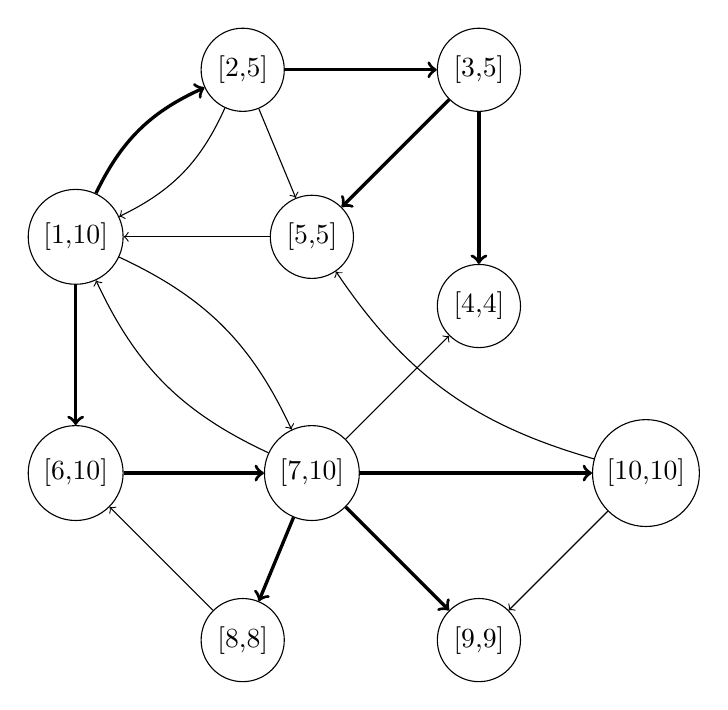
\begin{tikzpicture}[node distance=3cm]
    \node (1) [circle, draw] {[1,10]};
    \node (2) [circle, draw, above right of=1] {[2,5]};
    \node (3) [circle, draw, right of=2] {[3,5]};
    \node (4) [circle, draw, below of=3] {[4,4]};
    \node (5) [circle, draw, below left of=3] {[5,5]};
    \node (6) [circle, draw, below of=1] {[6,10]};
    \node (7) [circle, draw, right of=6] {[7,10]};
    \node (8) [circle, draw, below right of=6] {[8,8]};
    \node (9) [circle, draw, right of=8] {[9,9]};
    \node (10) [circle, draw, above right of=9] {[10,10]};

    \path[->] (2) edge [bend left=20] (1)
              (2) edge (5)
              (5) edge (1)
              (1) edge [bend left=20] (7)
              (7) edge [bend left=20] (1)
              (7) edge (4)
              (8) edge (6)
              (10) edge (9)
              (10) edge [bend left=20] (5);

    \path[->, very thick] (1) edge [bend left=20] (2)
              (2) edge (3)
              (3) edge (4)
              (3) edge (5)
              (1) edge (6)
              (6) edge (7)
              (7) edge (8)
              (7) edge (9)
              (7) edge (10);

\end{tikzpicture}
\end{figure}

$\forall u, v$ ci sono le due coppie di intervalli $[t(u), T(u)]$ e $[t(v), T(v)]$. I casi possibili sono tre:
\begin{enumerate}
    \item $[t(u), T(u)] \subseteq [t(v), T(v)]$
    \item $[t(u), T(u)] \supseteq [t(v), T(v)]$
    \item $[t(u), T(u)] \cap [t(v), T(v)] = \emptyset$
\end{enumerate}

Se $(u,v)$ \`e un arco, ci sono tre casi:
\begin{enumerate}
    \item $(u,v)$ ``passa dietro'' nella visita
    \item $(u,v)$ ``passa avanti'' nella visita
    \item $(u,v)$ \`e un arco di attraversamento. Deve essere che $t(u) > t(v)$.
\end{enumerate}

\begin{prop}
Sia $G$ un grafo diretto, $G$ \`e aciclico $\iff$ l'albero di visita DFS non ammette archi che ``passano dietro''.
\end{prop}

Siccome l'albero contiene sempre un cammino diretto da $u$ a tutti i vertici $v$ tali che si finisce con $v$ prima che si finisce con $u$, allora $(v,u)$ completa sempre un ciclo se $[t(u), T(u)] \supseteq [t(v), T(v)]$. 

Se $(u,v)$ \`e un arco \emph{non} nell'albero di visita, ci sono tre casi:
\begin{enumerate}
    \item $[t(u), T(u)] \cap [t(v), T(v)] = \emptyset \implies (u,v)$ \`e un arco di attraversamento. Un esempio nel grafo in figura  \ref{fig:visita_dfs} \`e l'arco (10,5). In questo caso deve essere che $t(u) > T(v)$. Quindi vediamo il nodo $u$ per la prima volta dopo aver visto il nodo $v$ per l'ultima volta.
    \item $[t(u), T(u)] \subseteq [t(v), T(v)]$, allora l'arco $(u,v)$ \`e un arco che ``torna indietro'', come l'arco (5,1) nel grafico in figura \ref{fig:visita_dfs}.
    \item $[t(u), T(u)] \supseteq [t(v), T(v)]$, allora l'arco $(u,v)$ \`e un arco ``in avanti'', come l'arco (1,7).
\end{enumerate}

Fino ad ora abbiamo visto un grafo diretto. Se il grafo indiretto, archi ``avanti'' e ``indietro'' coincidono. Inoltre, sempre se il grafo non \`e diretto, non esistono archi di attraversamento.

Gli archi di attraversamento portano da un nodo a un altro nodo contenuto su un sottoalbero diverso dal sottoalbero attuale dell'albero di visita.

Se un grafo non \`e diretto, e se $T$ \`e l'albero di visita di un algoritmo DFS, la presenza di archi ``all'indietro'' implica la presenza di un ciclo.

Per ogni coppia di vertici $(x,y)$ esiste un cammino che parte da $x$ e arriva a $y$ nell'albero di visita $T$. Se esiste un arco ``all'indietro'' $(x,y)$ che non appartiene all'albero di visita $T$, allora esiste un ciclo nel grafo $G$.

Quindi, se esiste un ciclo nel grafo $G$, allora $T$ ha un arco ``all'indietro''. Vale anche che, se $T$ non ha archi all'indietro, $G$ non ha cicli. Infatti, $T$ pu\`o avere solo archi all'indietro, essendo $G$ un grafo indiretto, e se non ne ha non pu\`o avere archi (l'albero di visita \`e un albero, quindi aciclico).

\begin{prop}
Sia $G$ un grafo indiretto, esiste un ciclo in $G \iff $ esiste un arco all'indietro nell'albero di visita DFS di $G$.
\end{prop}

Con i grafi diretti, non si pu\`o pi\`u dire che fra ogni coppia $(x,y)$ esiste un cammino da uno all'altro.

Prendiamo un generico arco $(y,x)$. Se $(y,x)$ \`e un arco all'indietro, come l'arco $(5,1)$ nella figura \ref{fig:visita_dfs}, allora esiste un ciclo diretto in $G$.

\begin{oss}
Tutti i vertici $y$ tali che $t(x) \le t(y) \le T(x)$ sono raggiungibili nell'albero di visita con un cammino diretto che parte da $x$ e arriva a $y$.
\end{oss}
\`E un po' una banalit\`a.

Se c'\`e un arco all'indietro, allora $[t(y), T(y)] \subseteq [t(x), T(x)]$, e quindi l'arco $(y,x)$ deve completare un ciclo diretto.

Dobbiamo far vedere anche che se esiste un arco all'indietro, deve esistere anche un ciclo nel grafo.

\begin{figure}
\centering
\begin{tikzpicture}
    \node (c0) [circle, draw, label=$c_0$] {};
    \node (c1) [circle, draw, label=$c_1$, below right = of c0] {};
    \node (c2) [circle, draw, label=$c_2$, below left = of c1] {};
    \node (c3) [circle, draw, label=$c_3$, left = of c2] {};
    \node (cn) [above left = of c3] {$\dots$};
    \node (ck) [circle, draw, label=$c_k$, above right = of cn] {};

    \path [->] (c0) edge (c1)
               (c1) edge (c2)
               (c2) edge (c3)
               (c3) edge (cn)
               (cn) edge (ck)
               (ck) edge (c0);
\end{tikzpicture}
\end{figure}

Prima di tutto, $t(c_0) \le t(c_i) \forall i \ge 1$. Ci sono archi che appartengono all'albero, ma non tutti sono archi all'indietro.

\begin{claim}
Per tutti gli indici $i \ge 1$, deve essere vero che $c_i$ viene completato prima della chiusira di $c_0$. Ossia, $T(c_i) \le T(c_0)$.
\end{claim}

\begin{proof}
Assumiamo per assurdo che esiste un $j$ tale che $T(c_j) \ge T(c_0)$, e sia $j$ proprio il valore minore per cui questo vale, allora vale che $T(c_{j-1}) \le T(c_0) \le T(c_j)$. Quindi $c_{j-1}$ viene visitato per l'ultima volta prima di aver visitato per l'ultima volta $c_j$. 

% grafico tempo con apertura e chiusura c_0 e c_{j-1}

Non pu\`o essere che $[t(c_j), T(c_{j})] \cap [t(c_{j-1}), T(c_{j-1})] \neq \emptyset$. Quindi o sono completamente disgiunti, ma $t(c_j)$ non pu\`o venire dopo $T(c_0)$, o sono contenuti uno nell'altro. Deve essere necessariamente che $[t(c_j), T(c_{j})] \supseteq [t(c_{j-1}), T(c_{j-1})]$, ma deve essere anche che $[t(c_j), T(c_{j})] \supseteq [t(c_{0}), T(c_{0})]$, poich\'e $T(c_{j-1})$ appartiene a entrambi. Siamo arrivati all'assurdo: non pu\`o essere che $t(c_j) \le t(c_0)$, perch\'e per ipotesi siamo partiti da $c_0$.
\end{proof}

Non abbiamo finito. Stiamo cercando un arco all'indietro. L'arco all'indietro \`e quello fra $(c_k, c_0)$. Abbiamo dimostrato che $T(c_k) \le T(c_0)$, e sappiamo inoltre che $t(c_0) \le t(c_k)$. Quindi $[t(c_k), T(c_k)] \subseteq [t(c_0), T(c_0)]$, e quindi c'\`e un arco all'indietro fra $(c_k, c_0)$.

\begin{prop}
Se esiste un ciclo diretto in un grafo $G$ diretto, esiste anche un arco all'indietro in un albero di visita DFS, e se esiste un arco all'indietro in un albero di visita DFS del grafo $G$, allora esiste un ciclo diretto nel grafo.
\end{prop}

C'\`e un modo semplice per memorizzare l'albero di visita: basta associare ad ogni vertice il vertice che l'ha scoperto. Quindi, se $u$ scopre il vertice $v$, per ricostruire l'albero basta memorizzare l'informazione che $u$ \`e il \emph{padre} di $v$. Per definizione il nodo radice non ha un padre, e questo si rappresenta con la convenzione $P(u) = u$, ossia il padre del nodo radice \`e il nodo stesso.

Per memorizzare l'albero di visita usiamo il vettore $P$ dei padri dei nodi. 

\begin{esercizio}
Dato in input il vettore $P$ dei padri, progettare un algoritmo che ricostruisce l'albero di visita come una lista di adiacenze.
\end{esercizio}

Si pu\`o usare il vettore per memorizzare se un nodo \`e o meno ancora dentro lo stack (ossia, deve essere analizzato). Se presumiamo che i vertici sono numerati con un intero da 1 a $n$, la prima volta che visitiamo un vertice $v$ (da un vertice $u$), settiamo $P[v] = -u$, e quando chiudiamo $u$ settiamo $P[v] = - P[v]$.

Se durante una visita DFS trovo un arco $(v,w)$, per sapere se l'arco \`e un arco che porta a un nodo gi\`a visitato devo controllare se $P[w] \neq 0$. Inoltre, $P[w] < 0$ se e solo se $(v,w)$ \`e un arco all'indietro. Quindi ora possiamo scrivere un algoritmo per trovare un ciclo in un grafo diretto tramite DFS.

\begin{algorithm}
\caption{Visita DFS per trovare un ciclo}
\begin{algorithmic}[1]
\State $P \gets$ vettore dei padri dei nodi inizializzato a 0
\Function{DFS\_CYCLE}{$G$ grafo, $v$ nodo, $u$ nodo, $P$ vettore}
    \State $P[v] \gets -u$
    \ForAll{$w$ adiacente a $v$}
        \If{$P[w] = 0$}
            \State $z \gets $ \Call{DFS\_CYCLE}{$G$, $w$, $v$, $P$}
            \If{$z \neq 0$}
                \State $P[v] \gets - P[v]$
                \State \Return $z$
            \EndIf
        \ElsIf{$P[w] < 0 \land (G$ diretto $\lor w \neq v)$}
            \State $P[w] = 0$
            \State $P[v] = u$
            \State \Return $v$
        \EndIf
        \State $P[v] = u$
        \State \Return $0$
    \EndFor
\EndFunction
\State $w \gets$ \Call{DFS\_CYCLE}{$G$, $u$, $u$, $P$}
\State $L \gets$ lista vuota
\While{$w > 0$}
    \State $L$.append($w$)
    \State $w \gets P[w]$
\EndWhile
\State \Return $L$
\end{algorithmic}
\end{algorithm}

$v$ \`e la radice, $u$ \`e il padre della radice. La funzione ritorna 0 se non trova nessun ciclo, un numero diverso da 0 se trova un ciclo.

Sia $G$ un grafo diretto senza cicli, vogliamo trovare un ordine topologico $x_1, x_2, \dots x_n$ in cui tutti gli archi sono $(x_i, x_j)$ con $x_i < x_j$. Una buona scelta per l'ultimo vertice dell'ordinamento \`e un nodo che non ha archi uscenti (che ci deve essere, lo sappiamo). Con un DFS ordiniamo i vertici partendo dall'ultimo, quello che viene ``chiuso'' per primo.

\subsection{Grafo di una citt\`a}

\begin{esercizio}
In un grafo diretto, i nodi rappresentano le intersezioni fra strade, e gli archi corrispondono alle strade. Un arco $f$ si dice \emph{arco critico} se $G - f$ non \`e pi\`u connesso. Il problema \`e determinare se un grafo ha un arco critico o meno.
\end{esercizio}

Si cancella l'arco $(u,v)$ e si controlla se si pu\`o ancora raggiungere $u$ da $v$. La complessit\`a \`e $O(m \cdot (n + m))$: un controllo DFS per tutti gli m archi.

Lo stesso algoritmo serve a trovare tutti i ponti in un grafo non diretto. Per\`o l'algoritmo \`e inefficiente. Proviamo a modificare il DFS per renderlo $O(n + m)$, nel caso in cui il grafo sia indiretto.

Fissiamo un vertice $v$ da cui costruire l'albero di visita DFS (con radice in $v$). Gli archi che non appartengono all'albero \emph{sicuramente} non sono ponti: anche eliminandoli si pu\`o sempre raggiungere tutto il grafo. Quindi se un arco \`e un ponte, l'arco appartiene a $E(T)$ (gli archi dell'albero di visita DFS). Ora il tempo \`e $O(n \cdot (n + m))$, controllando solo gli archi nell'albero (che sono $n$).

Consideriamo ora un arco $f = (u,w)$ all'interno dell'albero di visita, e chiamiamo $T(w)$ l'insieme di vertici che vengono dopo $w$ (nel sottoalbero con radice in $w$). Se esiste un arco all'indietro in $T(w)$ a un antenato di $u$ (o a $u$), allora $f$ non \`e un ponte. \`E un se e solo se: se esiste un ponte, allora esiste un arco all'indietro da $T(w)$ a un antenato di $u$ (o a $u$). O con altre parole, se $f$ non \`e un ponte esiste un cammino che porta da $u$ a $T(w)$, e quindi deve esserci un arco all'indietro da $T(w)$ a $u$.

Conclusione: un arco $f = (u,w)$ nell'albero DFS \`e un ponte $\iff$ non esiste un arco all'indietro con un termine dentro $V(T(w))$ e l'altro termine uguale a $u$ o un antenato di $u$.

\begin{algorithm}
\caption{Visita DFS per trovare un ponte}
\begin{algorithmic}[1]
\State $tt \gets$ array del momento della prima visita, inizializzato a 0
\State $c \gets$ contatore inizializzato a 0
\State $p \gets$ lista dei ponti, inizializzata a 0
\Function{DFS\_PONTE}{$G$ grafo, $u$ nodo, $z$ nodo, $tt$ array, $c$ intero, $p$ lista}
    \State $c \gets c + 1$
    \State $tt[u] \gets c$
    \State $back \gets c $
    \ForAll{$v \adj u$}
        \If{$tt[v] = 0$} (non \`e stato visitato)
            \State $b \gets$ \Call{DFS\_PONTE}{$G,v,u,tt,c,p$}
            \If{$b > tt[u]$}
                \State $p$.append($\{u,v\}$)
            \EndIf
            \State $back \gets \min(back, b)$
        \ElsIf{$v \neq z$}
            \State $back \gets \min(back, tt[v])$
        \EndIf
    \EndFor
    \State \Return $back$
\EndFunction
\end{algorithmic}
\end{algorithm}

\begin{defn}[Vertici di articolazione]
Un vertice di articolazione \`e un vertice $v$ tale per cui $G - v$ non \`e connesso.
\end{defn}
$G - v$ \`e il grafo senza il vertice $v$ e senza tutti gli archi incidenti a $v$.

Se $\{ u, v \}$ \`e un ponte incidente a $v$, $v$ \`e un vertice di articolazione $\iff \deg(v) = 2$.

Non vale l'inverso: se $v$ \`e un vertice di articolazione, gli archi incidenti a $v$ non sono necessariamente ponti. O anche: se esiste un vertice di articolazione, non necessariamente esiste un ponte.

Ora vogliamo usare un metodo simile a quello appena visto per trovare tutti i vertici di articolazione.

Sia $T$ l'albero DFS con radice $u$. Se $u$ ha un solo figlio, $u$ non \`e un vertice di articolazione, perch\'e qualunque cammino dentro l'albero fra due vertici non passer\`a mai per $u$, poich\'e dovrebbe passare due volte sullo stesso arco. Quindi, siccome esiste un cammino dal nodo $x$ al nodo $y$ in $T - u$, $T - u$ \`e connesso.

Se $u$ ha pi\`u di un figlio, perch\'e non sia un nodo di articolazione dovrebbe esistere un arco di attraversamento fra i sottoalberi individuati dai figli. Ma in un grafo indiretto tutti gli archi sono archi all'indietro, e mai archi di attraversamento, quindi $u$ \`e un nodo di articolazione.

Quindi, in conclusione, $u$ \`e un vertice di articolazione $\iff \deg_T (u) \ge 2$. Il tempo per trovare se un vertice \`e un nodo di articolazione \`e $O(n + m)$. Per trovare tutti i vertici di articolazione bisogna di nuovo usare una DFS modificata, per ottenere di nuovo un tempo $O(n+m)$.

\begin{algorithm}
\caption{Algoritmo per trovare i vertici di articolazione}
\begin{algorithmic}[1]
\State $tt \gets$ vettore del momento della prima visita, inizializzato a 0
\State $c \gets 0$
\State $A \gets$ insieme vuoto di vertici di articolazione
\Function{DFS\_ART}{$G$ grafo, $v$ nodo, $tt$, $c$, $A$}
    \State $c \gets c + 1$
    \State $tt[v] \gets c$
    \State $children \gets 0$
    \State $back \gets c$
    \ForAll{$w \adj v$}
        \If{$tt[w] = 0$}
            \State $children \gets children + 1$
            \State $b \gets$ \Call{DFS\_ART}{$G, w, tt, c, A$}
            \If{$tt[v] > 1 \land b \ge tt[v]$} (non vale per la radice)
                \State $A$.add($v$)
            \EndIf
            \State $back \gets \min(back, b)$
        \Else
            \State $back \gets \min(back, tt[w])$
        \EndIf
    \EndFor
    \If{$tt[v] = 1 \land children \ge 2$}
        \State $A$.add($v$)
    \EndIf
    \State \Return $back$
\EndFunction
\end{algorithmic}
\end{algorithm}

\begin{defn}[Nodo critico]
Dati due nodi $a$ e $b$, un nodo $c$ diverso da $a$ e da $b$ si dice critico per $a$ e $b$ se ogni cammino da $a$ a $b$ contiene $c$.
\end{defn}

Per controllare se un dato nodo $x$ \`e un nodo critico per un paio di vertici $a, b$ basta controllare se esiste un cammino da $a$ a $b$ in $G - x$.

Per avere tutti i nodi critici dati due nodi $a$ e $b$, si potrebbe controllare ogni altro vertice, ma il tempo sarebbe $O(n \cdot (n + m))$.

\begin{oss}
Dati due vertici $a$ e $b$ e un vertice $c$ critico per $a$ e $b$, $c$ \`e un vertice di articolazione, perch\'e $a$ appartiene a un componente di $G - c$ e $b$ appartiene a un componente di $G - x$, e questi componenti devono essere distinti perch\'e non c'\`e nessun cammino da $a$ a $b$.
\end{oss}

Non vale l'inverso: un vertice di articolazione non \`e un nodo critico per due vertici $a$ e $b$.

Abbiamo un algoritmo per trovare tutti i vertici di articolazione in tempo $O(n + m)$. Possiamo notare che, dato un qualsiasi cammino $P$ da $a$ a $b$, tutti i vertici critici per $a$ e $b$ (se ci sono) devono essere in questo cammino.

Un grafo \`e biconnesso se per ogni vertice $x$, $G - x$ \`e connesso. Un componente biconnesso \`e un sottografo massimale che \`e biconnesso. Un ciclo \`e sempre biconnesso. Dobbiamo modificare il DFS visto l'ultima volta per trovare tutti i componenti biconnessi. Un vertice in comune fra componenti biconnessi \`e sempre un vertice di articolazione. I nodi critici sono i vertici di articolazione fra i componenti biconnessi contenenti $a$ e $b$.

\subsection{Forte connettivit\`a in grafi diretti}

Per determinare se un grafo diretto \`e fortemente connesso, potrei $\forall u \in V (G)$ fare un $\operatorname{DFS}(G,u)$ e se esiste un vertice $v$ non connesso a $u$, ritornare falso, altrimenti ritornare vero. Ma il tempo \`e esagerato: $O(n \cdot (n + m))$.

Il grafo trasposto $G^T$ \`e il grafo con l'orientamento di tutti gli archi invertito. Per determinare se per tutti i vertici $v$ esiste un cammino da $v$ a $u$, basta fare un $\operatorname{DFS}(G^T, u)$. Quindi l'algoritmo \`e:

\begin{algorithm}
\caption{Test per la forte connettivit\`a in un grafo diretto}
\begin{algorithmic}[1]
    \State fisso un vertice $u$
    \State $T_1 \gets$ l'albero di ricerca del $\operatorname{DFS}(G, u)$
    \State $T_2 \gets$ l'albero di ricerca del $\operatorname{DFS}(G^T, u)$
    \If{$V(T_1) = V(T_2) = V(G)$}
        \State \Return TRUE
    \Else
        \State \Return FALSE
    \EndIf
\end{algorithmic}
\end{algorithm}

\begin{prop}
Sia $G$ un grafo diretto e sia $u \in V(G)$, $T_1$ l'albero di ricerca di $\operatorname{DFS}(G, u)$ e $T_2$ l'albero di ricerca $\operatorname{DFS}(G^T, u)$, $G$ \`e fortemente connesso $\iff V(T_1) = V(T_2) = V(G)$.
\end{prop}

Infatti, dati comunque due vertici $x, y \in V(G)$, esiste un cammino da $x$ a $u$ e un cammino da $u$ a $y$, e quindi esiste una ``passeggiata'' da $x$ a $y$. (Si chiama passeggiata, e non cammino, perch\'e pu\`o essere un cammino che passa pi\`u volte sugli stessi nodi)

Se volessimo trovare i componenti fortemente connessi di un grafo? Abbiamo visto che i grafi biconnessi possono intersecarsi, ma i componenti fortemente connessi non possono avere intersezione non vuota.

\begin{defn}[Componente fortemente connesso]
Un componente fortemente connesso di un grafo $G$ \`e un sottografo massimale fortemente connesso.
\end{defn}

Siano $U_1$ e $U_2$ insiemi di vertici di componenti fortemente connessi, allora $U_1 \cap U_2 = \emptyset$, altrimenti per $x, y \in U_1 \cup U_2$ esiste un cammino da $x$ a un vertice appartenente a $U_1 \cap U_2$, e un cammino da questo vertice a $y$, e quindi esiste un cammino da $x$ a $y$.

Fissiamo un nodo $u$ e cerchiamo il componente che contiene questo nodo.
\begin{align*}
T_1 &= \operatorname{DFS}(G, u) \\
T_2 &= \operatorname{DFS}(G^T, u)
\end{align*}
Il componente fortemente connesso contenente $u$, per gli stessi motivi di prima, \`e $V(T_1) \cap V(T_2)$. Infatti ciascuna coppia di vertici in $V(T_1) \cap V(T_2)$ \`e fortemente connessa, e ciascun nodo all'esterno dell'intersezione non \`e fortemente connesso. Il tempo per trovare questo componente fortemente connesso per\`o \`e $O(n \cdot (n + m))$.

Diamo qualche definizione.

\begin{defn}
Il sottografo indotto su un insieme di vertici $X$ \`e il sottografo con vertici in $X$ e tutti gli archi di $G$ con entrambi i termini dentro $X$. Si indica con $G[X]$.
\end{defn}

Siano $G[U_1]$ e $G[U_2]$ due sottografi indotti fortemente connessi, con un arco da $U_1$ a $U_2$ e un arco da $U_2$ a $U_1$, allora $G[U_1 \cup U_2]$ \`e un sottografo indotto fortemente connesso.

\begin{defn}
Per contrarre un insieme di vertici $X$ in un grafo, tolgo $X$ e aggiungo un vertice nuovo $V_X$ e per ogni arco $(z,y)$ o $(y,z)$ con $z \in X$ e $y \notin X$ aggiungo un arco da $V_X$ a $y$ o da $y$ a $V_X$. Il grafo contratto si scrive $G / X$.
\end{defn}

\begin{figure}
\centering
\caption{Grafo contratto}
\begin{tikzpicture}[node distance=1.5cm]
    \node (A1) [circle, draw] {}; 
    \node (A2) [circle, draw, above right = of A1] {}; 
    \node (A3) [circle, draw, below right = of A1] {}; 
    \node (A4) [circle, draw, below right = of A2] {};

    \node (A5) [circle, draw, above right = of A2] {}; 
    \node (A9) [circle, draw, below right = of A3] {}; 

    \node (A6) [circle, draw, right = of A5] {}; 
    \node (A8) [circle, draw, right = of A9] {}; 
    \node (A7) [circle, draw, right = 3.5cm of A4] {}; 

    \path[->]   (A1) edge [bend left=20] (A2)
                (A2) edge [bend left=20] (A4)
                (A3) edge [bend left=20] (A1)
                (A4) edge [bend left=20] (A3)
                (A2) edge (A5)
                (A5) edge (A6)
                (A6) edge (A7)
                (A7) edge (A8)
                (A8) edge (A9)
                (A9) edge (A3);

    \node (B1) [circle, draw, right = of A7] {$V_X$}; 

    \node (B5) [circle, draw, above right = of B1] {}; 
    \node (B9) [circle, draw, below right = of B1] {}; 

    \node (B6) [circle, draw, right = of B5] {}; 
    \node (B8) [circle, draw, right = of B9] {}; 
    \node (B7) [circle, draw, below right = of B6] {}; 

    \path[->]   (B1) edge (B5)
                (B5) edge (B6)
                (B6) edge (B7)
                (B7) edge (B8)
                (B8) edge (B9)
                (B9) edge (B1);
\end{tikzpicture}
\end{figure}

\begin{prop}
Sia $U$ un insieme di vertici tali per cui il sottografo indotto $G[U]$ \`e fortemente connesso, se $G / U$ \`e fortemente connesso, allora anche $G$ \`e fortemente connesso.
\end{prop}

Creiamo un nuovo algoritmo: in input prende un grafo $G$, e in output d\`a una lista $\{ U_1, U_2, \ldots, U_l \}$ dei componenti fortemente connessi.

\begin{algorithm}
\caption{Come \emph{non} trovare i componenti fortemente connessi}
\begin{algorithmic}[1]
\Function{Fort}{$G$ grafo}
    \State trova un ciclo $C$ in $G$
    \If{non esiste un ciclo $C$}
        \State \Return $(\{ v \} : v \in V(G))$
    \EndIf
    \State $\{ U_1, \ldots, U_l \} \gets$ \Call{Fort}{G / C}
    \ForAll{$U_i \in \{U_1, \ldots, U_l \}$}
        \If{$V_C \in U_i$}
            \State $U_i' \gets (U_i - V_C) \cup V(C)$
        \Else
            \State $U_i' \gets U_i$
        \EndIf
    \EndFor
    \State \Return $\{ U_1', \ldots, U_l' \}$
\EndFunction
\end{algorithmic}
\end{algorithm}

La ricorsione pu\`o esser fatta al massimo $O(n)$ volte, poich\'e $G$ decresce ad ogni passo. Ad ogni passo, ci vuole $O(n + m)$ per trovare un ciclo. Quindi il tempo totale pu\`o essere maggiorato con $O(n \cdot (n + m))$. Che non \`e un tempo ottimale.

\section{Componenti fortemente connessi}

\begin{defn}[C-radice]
Una C-radice \`e il primo nodo trovato in un componente fortemente connesso durante un dato DFS.
\end{defn}

\begin{prop}
Un nodo $u$ non \`e una C-radice $\iff$ nella chiamata ricorsiva del $DFS$ con radice $u$ viene attraversato un arco $(v,w)$ tale che il nodo $w$ \`e gi\`a stato visitato (quindi $t[w] < t[u]$) e il componente di $w$ non \`e ancora stato determinato.
\end{prop}

\begin{proof}
Se $u$ non \`e una C-radice, la C-radice per il componente fortemente connesso contenente $u$ si trova \emph{prima} di $u$ nell'albero di visita DFS (ossia, \`e gi\`a stato visitato). Quindi esiste un cammino da $u$ alla C-radice di $C(u)$, e in questo cammino deve esserci un arco $(v',w')$ che ritorna ad un vertice gi\`a visitato. Essendo $w'$ nello stesso componente $C(u)$, vuol dire che il componente di $w'$ non \`e ancora stato trovato.

Nell'altro senso, supponiamo $u$ sia una C-radice, ma esiste un arco $(v,w)$ ad un nodo $w$ visitato prima di $u$ nella $DFS$ (e il cui componente fortemente connesso non \`e ancora stato determinato). Sia $z$ la C-radice di $C(w)$. Il nodo $z$ deve essere un antenato di $u$: se il componente $C(w)$ non \`e stato stabilito, allora $C(z)$ non \`e stato ancora stabilito. $z$ \`e ancora aperto nel $DFS$, ma gli unici vertici ancora aperti sono gli antenati di $u$. La contraddizione \`e nel fatto che esiste un cammino da $u$ a $v$, perch\'e $v$ viene scoperto nel $DFS$ partendo da $u$. Esiste poi un arco da $v$ a $w$, e un cammino da $w$ a $z$, essendo $w \in C(z) = C(w)$, e un cammino da $z$ a $u$ essendo $z$ un antenato di $u$. Quindi $u \in C(z)$, ma $z$ \`e la C-radice di $C(z)$.
\end{proof}

Basta mantenere un $back(u)$ che ricorda l'arco pi\`u all'indietro a un vertice per il quale non \`e stato ancora stabilito il componente fortemente connesso.

\begin{itemize}
    \item $Comp[u] =$ inizializzato a 0 per tutti i nodi $u$
    \item $Comp[u] = - t(u)$ la prima volta che incontriamo $u$
    \item $Comp[u] =$ numero dei componenti quando troviamo tutti i vertici di $C(u)$
\end{itemize}

\begin{algorithm}
\caption{Trovare i componenti fortemente connessi}
\begin{algorithmic}[1]
\Function{SCC}{$G$ grafo}
    \State $Comp \gets$ array inizializzato a 0
    \State $nc \gets$ contatore dei componenti
    \State $c \gets$ contatore per la visita
    \State $S \gets$ uno stack
    \ForAll{$u \in V(G)$}
        \If{$Comp[u] = 0$}
            \State \Call{DFS\_SCC}{$G, u, Comp, S, c, nc$}
        \EndIf
    \EndFor
    \State \Return $Comp$
\EndFunction
\end{algorithmic}
\end{algorithm}

\begin{algorithm}
\caption{Visita DFS per trovare i componenti fortemente connessi}
\begin{algorithmic}[1]
\Function{DFS\_SCC}{$G$ grafo, $u$ nodo, $Comp$ array, $S$ stack, $c$ contatore, $nc$ contatore}
    \State $c \gets c + 1$
    \State $Comp[u] \gets -c$
    \State $S$.push($u$)
    \State $back \gets c$
    \ForAll{$v \adj u$}
        \If{$Comp[v] = 0$}
            \State $b \gets$ \Call{DFS\_SCC}{$G, v, Comp, S, c, nc$}
            \State $back \gets \min(back, b)$
        \EndIf
        \If{$Comp[v] < 0$}
            \State $back \gets \min(back, -Comp[v])$
        \EndIf
    \EndFor
    \If{$back = - Comp[u]$}
        \State $nc \gets nc + 1$
        \Repeat
            \State $w \gets S$.pop()
            \State $Comp[w] \gets nc$
        \Until{$w \neq u$}
    \EndIf
    \State \Return $back$
\EndFunction
\end{algorithmic}
\end{algorithm}

\section{Best Friend Search}
\label{sezione_visita_bfs}

Il $DFS$ \`e utile per vedere se esiste un cammino da un nodo $u$ a un nodo $v$, ma non se voglio trovare il cammino pi\`u breve da $u$ a $v$. L'idea del $BFS$ \`e di partire da un nodo e controllare prima i vicini di quel nodo, e ripetere poi l'operazione ricorsivamente.

Sia $G$ un grafo, $dist(u,v)$ \`e la lunghezza minima di un cammino da $u$ a $v$, dove la lunghezza di un cammino \`e il numero degli archi del cammino.

\begin{prop}
Se $dist(u,v) = k$ e $w \adj v$, allora $dist(u,w)$ \`e:
\[
k - 1 \le dist(u,w) \le k + 1
\]
\end{prop}

\begin{proof}
\`E al massimo $k+1$, perch\'e se $P$ \`e il cammino da $u$ a $v$ di lunghezza $k$, allora $P + (v,w)$ \`e una ``passeggiata'' da $u$ a $w$ di lunghezza $k+1$.

Se esistesse un cammino $P$ di lunghezza $h < k - 1$ da $u$ a $w$, allora esiste un cammino $P + (w,v)$ di lunghezza $h + 1 < k$, in contraddizione con l'ipotesi che la distanza da $u$ a $v$ \`e $k$.
\end{proof}

\begin{defn}
Un cammino \`e una serie $v_0 e_1 v_1 e_2 v_2 \ldots e_k v_k$ dove $e_i = (v_{i-1}, v_i)$ e $v_i \neq v_j \forall i \neq j$. Per una passeggiata \`e invece permesso che $v_i = v_j$.
\end{defn}

\begin{algorithm}
\caption{Visita $BFS$}
\begin{algorithmic}[1]
\Function{BFS}{$G$ grafo, $u$ nodo}
    \State $P \gets$ vettore dei padri
    \State $Dist \gets$ array delle distanze
    \State $P[u] \gets u$
    \State $Dist[u] \gets 0$
    \State $Q \gets$ coda FIFO dei vertici aperti
    \State $Q$.enqueue($u$)
    \While{$Q \neq \emptyset$}
        \State $v \gets Q$.dequeue()
        \For{$w \adj v$}
            \If{$P[w] = 0$}
                \State $P[w] \gets v$
                \State $Q$.enqueue($w$)
                \State $Dist[w] \gets Dist[v] + 1$
            \EndIf
        \EndFor
    \EndWhile
    \State \Return $Dist, P$
\EndFunction
\end{algorithmic}
\end{algorithm}

\section{Grafi pesati}

Un grafo \`e pesato quando esiste una funzione $p : E(G) \to \reals^{+}$, che associa a ciascun arco un numero reale (positivo). Il peso di un cammino \`e la somma dei pesi dei singoli archi:
\[
p(C) = \sum_{c \in E(C)} p(c)
\]
La distanza fra due vertici $u$ e $v$ ora \`e il peso del cammino con peso minimo.
\[
dist(u,v) = \min_{C \text{ cammino da } u \text{ a } v} p(C)
\]
\begin{oss}
Due rapide osservazioni:
\begin{align*}
dist(u,u) & = 0 \\
dist(u,v) & \ge 0
\end{align*}
\end{oss}

In generale vale questa disuguaglianza:
\[
p(u,w) \le p(u,v) + p(v,w)
\]
Il percorso che va da $u$ a $v$ e poi da $v$ a $w$ non \`e detto sia il percorso minimo da $u$ a $w$.

In un grafo indiretto, vale sempre che $dist(u,v) = dist(v,u)$.

Problema: dato un grafo pesato $G$ vogliamo trovare il cammino con peso minimo da un nodo $u$ a un nodo $v$.

Ripensiamo al $BFS$. Da un nodo, controllavamo tutti i nodi vicini, finch\'e non scopriamo tutto il grafo. Ora, partendo da un nodo $u$, vogliamo trovare la distanza minima di tutti i nodi nel grafo.

Partendo dal nodo $u$, consideriamo il suo vicino $w$ con peso minore sull'arco $(u,w)$. Questo sar\`a proprio il cammino minimo da $u$ a $w$. Infatti:
\[
p(u,w) \le p(u,v') \implies p(u,w) \le p(u,v') + p(v',w)
\]
Questo perch\'e il peso \`e sempre tale che $p(v',w) \ge 0$.

Abbiamo fatto il passo base, ora facciamo un po' di ricorsione. Assumiamo di avere un insieme di vertici $R$ per i quali conosciamo gi\`a la distanza da $u$. Possiamo aggiungere a $R$ il nodo $w$ tale per cui $dist(u,r) + p(r,w)$ \`e minimo, al variare di $r \in R$.

Se, infatti, $w$ \`e il nodo (non ancora in $R$) tale per cui $dist(u,r) + p(r,w)$ \`e minima, allora la distanza \`e $dist(u,w) = dist(u,r) + p(r,w)$.

\begin{proof}
Boh:
\[
dist(u,w) \le dist(u,r) + dist(r,w) \le dist(u,r) + p(r,w)
\]
Viceversa, sia $C$ un cammino da $u$ a $w$, vogliamo dimostrare che $p(C) \ge dist(u,r) + p(r,w)$. Se $C$ passa per il vertice $r$, allora evidentemente:
\[
p(C) = p(uCr) + p(rCw) \ge dist(u,r) + dist(r,w)
\]
Consideriamo il primo arco $(r',v')$ nel cammino $C$ tale per cui $r'$ \`e dentro $R$ e $v'$ no. Vale questo:
\[
p(C) \ge dist(u,r') + p(r',v') \ge dist(u,r) + p(r,w)
\]
L'ultima parte \`e ci\`o che stavamo minimizzando. Fine.
\end{proof}

\subsubsection{Un primo algoritmo di Dijkstra}

\begin{algorithm}
\caption{\label{dijkstra}Algoritmo di Dijkstra per trovare i percorsi minimi}
\begin{algorithmic}[1]
\Function{Dijkstra}{$G$ grafo, $u$ nodo, $p$ funzione peso}
    \State $Dist \gets$ array inizializzato a $-1$
    \State $P \gets$ vettore dei padri
    \State $R \gets$ insieme di vertici di cui si conosce la distanza minima
    \State $Dist[u] \gets 0$
    \State $P[u] \gets u$
    \State $R \gets R \cup \{ u \}$
    \While{esiste un arco da un nodo in $R$ a un nodo fuori di $R$}
        \State trova un arco $(v,w)$ tale che $v \in R$ e $w \notin R$ per cui $Dist[v] + p(v,w)$ \`e minimo
        \State $Dist[w] \gets Dist[v] + p(v,w)$
        \State $P[w] \gets v$
        \State $R \gets R \cup \{ w \}$
    \EndWhile
    \State \Return $Dist, P$
\EndFunction
\end{algorithmic}
\end{algorithm}

Il tempo, per come \`e fatto l'algoritmo \ref{dijkstra}, \`e $O(n \cdot m)$. Si pu\`o fare di meglio.

In realt\`a, oltre all'insieme dei vertici $R$, abbiamo una ``frontiera'' $F$ di nodi raggiungibili direttamente (con un solo arco) da $R$. Per ciascun vertice $w$ in questa frontiera $F$, memorizziamo il valore minimo $dist(u,r) + p(r,w)$ per un certo $r$. Rifacendo questo controllo ogni volta che cambia, il lavoro fatto all'interno del ciclo \code{while} \`e $O(\deg(v))$, ossia dipende dal grado del nodo.

Per memorizzare la frontiera conviene usare un min-heap.

\subsubsection{Il vero algoritmo di Dijkstra}

\begin{algorithm}
\caption{\label{truedijkstra}Il vero algoritmo di Dijkstra: diffidate delle imitazioni}
\begin{algorithmic}[1]
\Function{TrueDijkstra}{$G$ grafo, $u$ nodo, $p$ funzione di peso}
    \State $Dist \gets$ array inizializzato a $\infty$
    \State $P \gets$ vettore dei padri
    \State $H \gets$ min-heap inizializzato con tutti i nodi, le priorit\`a sono i valori di $Dist$
    \State $Dist[u] \gets 0$
    \State $P[u] \gets u$
    \While{$H \neq \emptyset$}
        \State $v \gets H$.getmin()
        \ForAll{$w \adj v$}
            \If{$Dist[w] \ge Dist[v] + p(v,w)$}
                \State $Dist[w] \gets Dist[v] + p(v,w)$
                \State $P[w] \gets v$
                \State $H$.decrease($w$)
            \EndIf
        \EndFor
    \EndWhile
    \State \Return $Dist, P$
\EndFunction
\end{algorithmic}
\end{algorithm}

Durante l'esecuzione dell'algoritmo \ref{truedijkstra}, la frontiera $F$ \`e l'insieme di nodi $w$ ancora in $H$ tali per cui $Dist[w] < \infty$.

La complessit\`a \`e $O(n \cdot \log(n))$ per inizializzare il min-heap. Poi, ogni volta che si estrae il minimo, il tempo \`e $O(\log(n))$. Il tempo \`e $O(\log(n))$ anche per il \code{decrease}. Il ciclo \code{for} interno viene fatto $\deg(v)$ volte. Quindi il numero di volte che il ciclo \code{while} viene fatto \`e:
\[
\sum \deg(v) \cdot \log(n) = O(m \cdot \log(n))
\]
Quindi in totale il tempo \`e $O((n + m) \cdot \log(n))$.

\subsection{Problemi sui grafi pesati}

Sia $G$ un grafo, $u \in V(G)$ un vertice, e $p: E(G) \to \reals^{+}$ una funzione di peso.

$T$ \`e l'albero di cammini di peso minimo trovato con l'algoritmo di Dijkstra. Sia $p' : E(G) \to \reals^{+}$ la funzione:
\[
p'(e) = p(e) + 1
\]
Ci chiediamo, \`e vero che $T$ \`e un albero di cammini di peso minimo anche rispetto alla funzione $p'$? Non sempre.

% disegnare grafico
% quattro nodi
% quattro archi, tre con peso 1 e uno con peso 4

Se invece definiamo $p''(e) = 2 \cdot p(e)$, l'albero di cammini di peso minimo resta un albero di cammini di peso minimo.

Nel primo caso, il nuovo peso dipende dal numero di archi nel cammino, mentre nel secondo caso no.
\[
p''(C) = \sum_{e \in E(C)} p''(e) = \sum_{e \in E(C)} 2 \, p(e) =
2 \, \sum_{e \in E(C)} p(e) = 2 \, p(C)
\]
Se $P_T$ \`e un cammino dentro l'albero $T$, allora il suo nuovo peso \`e $p''(P_T) = 2 \, p(P_T) \le 2 \, p(C) = p''(C)$. Quindi $P_T$ \`e rimasto un cammino di peso minimo, maggiorato dal peso di ogni altro cammino $C$.

\subsection{Algoritmi greedy}

L'algoritmo di Dijkstra fa parte di una famiglia di algoritmi chiamati ``greedy''. Ad ogni passo dell'algoritmo, si sceglie un unico nodo da aggiungere all'albero fra tutti i nodi disponibili, e quel nodo \`e il nodo ``migliore''.

In generale:
\begin{itemize}
    \item al passo $i$-esimo abbiamo una soluzione parziale $S_i$
    \item controlliamo tutti gli elementi rimasti
    \item scegliamo l'elemento $x$ ``pi\`u conveniente''
    \item $S_{i+1} = S_i \cup \{ x \}$
\end{itemize}

\begin{exmp}
Consideriamo in input un insieme di intervalli ``mezzi chiusi'', ossia nella forma $\coint{a_i}{b_i}$.

% disegnare serie di intervalli

Vogliamo trovare un sottoinsieme massimo (di massima cardinalit\`a) di intervalli disgiunti.

Cosa vuol dire ``pi\`u conveniente'' in questo contesto?
\begin{enumerate}
    \item L'intervallo pi\`u corto? No, se l'intervallo pi\`u corto interseca due intervalli pi\`u lunghi.
    \item L'intervallo che interseca il minor numero di altri intervalli? Forse.
    \item L'intervallo che inizia per primo? C'\`e per\`o il problema che se l'intervallo che inizia per primo finisce per ultimo, perdiamo tutti gli altri intervalli. Quindi questo non va bene.
    \item L'intervallo che finisce per primo?
\end{enumerate}

\begin{algorithm}
\caption{Algoritmo per trovare la roba che stiamo cercando}
\begin{algorithmic}[1]
\Function{TerminaPrima}{$S$ insieme di intervalli}
    \State $Sol \gets \emptyset$
    \While{$\exists$ un intervallo che non interseca gli intervalli di $Sol$}
        \State trovare un intervallo $\coint{a_i}{b_i} \in S$ che non interseca gli intervalli di $Sol$ e con $b_i$ minimo
        \State $Sol \gets Sol \cup \{ \coint{a_i}{b_i} \}$
    \EndWhile
    \State \Return $Sol$
\EndFunction
\end{algorithmic}
\end{algorithm}

C'\`e un approccio generale per dimostrare la correttezza degli algoritmi greedy. Si dimostra che ogni soluzione parziale porta dopo un certo numero di passi a una soluzione ottimale.

Abbiamo una serie di soluzioni $S_0, S_1, S_2, \ldots S_n$, dove $S_{i} \subseteq S_{i+1}$, e $S_{i+1}$ \`e ottenuto da $S_i$ aggiungendo l'elemento pi\`u conveniente.

Per dimostrare in generale che l'algoritmo \`e giusto (ossia che trova la soluzione ottimale), basta dimostrare che per ogni $i \ge 0$ esiste una soluzione ottimale $S^{o} \supseteq S_i$.

\begin{prop}
Se \`e vero che per ogni $i \ge 0$ esiste una soluzione ottimale $S^{o} \supseteq S_i$, allora l'algoritmo trova la soluzione ottimale.
\end{prop}

\begin{proof}
L'algoritmo deve terminare con una soluzione parziale $S_m$. Se l'algoritmo non \`e corretto, allora $S_m \neq S^{o}$, o meglio esiste una soluzione $S^{o}$ migliore di $S_m$.

Per la proposizione, per\`o, possiamo assumere che $S^{o} \supseteq S_m$. Quindi esiste $x \in S^{o} \setminus S_m$, ma al passo per trovare $S_{m+1}$ non c'era nessun elemento da aggiungere a $S_m$. Contraddizione. 
\end{proof}

Come si dimostra che per ogni $i \ge 0$ esiste una soluzione ottimale $S^{o} \supseteq S_i$?

\begin{proof}
Per induzione, $S_0 = \emptyset$, e ovviamente esiste una soluzione ottimale che contiene $S_0$.

Assumiamo che $S_h \subseteq S^{o}$ per dimostrare che esiste una soluzione $S^{o}_2 \supseteq S_{h+1}$. $\exists x$ tale che $S_{h+1} = S_h + \{ x \}$.

Se $x \in S^{o}$, non abbiamo pi\`u niente da dimostrare. Quindi consideriamo il caso in cui $x \notin S^{o}$. Se esiste un $y$ tale per cui $(S^{o} - y) \cup \{ x \}$ \`e ottimale, abbiamo finito. 
\end{proof}

Nel caso dell'algoritmo, al passo $h$ esiste un intervallo $x$ disgiunto da tutti gli intervalli di $S_h$, e che finisce per primo. Se $x$ fosse disgiunto anche dagli intervalli della soluzione ottimale, avremmo una contraddizione, poich\'e dovrebbe essere dentro la soluzione ottimale.

$x$ non pu\`o neanche intersecare \emph{pi\`u di un} intervallo dentro $S^{o}$, perch\'e \`e l'intervallo che termina prima.

Quindi:
\begin{prop}
$x$ interseca \emph{al massimo} un intervallo di $S^{o} \setminus S_h$.
\end{prop}

\begin{proof}
Altrimenti, $\exists \coint{a_j}{b_j}$ e $\coint{a_l}{b_l}$ in $S^{o} \setminus S_h$ che intersecano $x$. $\coint{a_j}{b_j}$ e $\coint{a_l}{b_l}$ sono disgiunti. Assumiamo che $b_j \le a_l$. Se $x$ interseca entrambi, allora $\coint{a_j}{b_j}$ finisce prima di $x$. Contraddizione.
\end{proof}

L'intervallo che interseca $x$ \`e il nostro $y \in S^{o} - S_h$, e $(S^{o} - y) \cup \{ x \}$ \`e la nuova soluzione ottimale.
\end{exmp}

\subsection{Correttezza dell'algoritmo di Dijkstra}

\begin{algorithm}
\caption{\label{algoritmo_dijkstra_semplice}Algoritmo di Dijkstra semplificato}
\begin{algorithmic}[1]
\Function{Dijkstra}{$G$ grafo, $u$ nodo}
    \State $Dist \gets$ array delle distanze iniziato a $\infty$
    \State $Dist[u] \gets 0$
    \State $R \gets \{ u \}$
    \While{esiste un arco fuori da $R$}
        \State trova un arco $(v,w)$ con $v \in R$ e $w \notin R$ che minimizza $Dist[v] + p(v,w)$
        \State $Dist[w] \gets Dist[v] + p(v,w)$
        \State $R \gets R \cup \{ w \}$
    \EndWhile
    \State \Return $Dist$
\EndFunction
\end{algorithmic}
\end{algorithm}

Con l'algoritmo \ref{algoritmo_dijkstra_semplice}, le soluzioni parziali sono rappresentate dai valori dell'array $Dist$. 

Per dimostrare la correttezza di Dijkstra, bisogna dimostrare che dopo $h$ passi per tutti i vertici $v$ con $Dist[v] < \infty$ esiste una soluzione ottimale che ha gli stessi valori di $Dist$.

Il caso base \`e dimostrato banalmente. Per induzione, ora, dobbiamo dimostrare che dopo che abbiamo stabilito i primi $h$ valori, quando prendiamo il valore $h+1$ \`e il valore giusto. Quindi, se aggiungiamo un nodo $w$, dobbiamo dimostrare che $dist(u,w) = Dist[v] + p(v,w)$. E l'abbiamo visto prima.

\section{Minimum spanning tree}

\begin{esercizio}
Abbiamo un grafo non connesso. Sappiamo i costi che avrebbero gli archi fra certi nodi. Vogliamo scegliere l'insieme di archi che rende il grafo connesso, e che ha costo minimo.

Quindi: dato un grafo G non diretto con pesi p : E(G) \to \reals^{+}, vogliamo trovare il costo di un sottografo connesso di costo minimo.
\end{esercizio}

\begin{oss}
Se H \`e un sottografo connesso di costo minimo \implies H \`e un albero.
\end{oss}

Non abbiamo definito bene cosa \`e un albero: un albero \`e un grafo connesso senza cicli.

\begin{proof}
Per ipotesi, H \`e connesso. Quindi, se H non \`e un albero, deve avere un ciclo. Ma togliendo un qualsiasi arco (u,v) appartenente a un ciclo da un grafo connesso contenente un ciclo, abbiamo ancora un grafo connesso, ma aciclico. Ossia, ogni cammino x \to y in H - (u,v) pu\`o essere ridiretto nel ciclo per arrivare da x a y senza l'arco (u,v).

H era un sottografo di peso minimo connesso, ma H - (u,v) \`e connesso e p(H - (u,v)) < p(H). Contraddizione.
\end{proof}

Il problema quindi \`e trovare un albero che copre tutto il grafo e che ha costo minimo sugli archi. L'algoritmo di Kruskal inizia con Sol = \emptyset, e si aggiunge a Sol l'arco $e$ di peso minimo, a patto che Sol + e non contenga un ciclo.

La complessit\`a di questo algoritmo non \`e banale. Per ogni arco fra due nodi (u,v), bisogna controllare che non ci sia un ciclo. Con un BFS ci vorrebbe O(n+m).

C'\`e un modo pi\`u semplice da dimostrare.

\begin{algorithm}
\begin{algorithmic}
\Function{Prim}{G non diretto, pesato e connesso}
    \State Sol \gets \emptyset
    \State s \gets un nodo in V(G)
    \State C \gets \{ s \}
    \While{C \neq V(G)}
        \State sia (u,v) un arco di peso minimo con u \in C e v \ni C
        \State C \gets C + \{ v \}
        \State Sol \gets Sol + (u,v)
    \EndWhile
    \Return Sol
\EndFunction
\end{algorithmic}
\end{algorithm} 

\begin{proof}[dell'algoritmo]
Chiamiamo Sol_i la soluzione al passo i-esimo del ciclo. \forall i \ge 0, esiste una soluzione ottimale Sol^{o} \supseteq Sol_i. Il caso base \`e banale: \emptyset \subseteq Sol^{o}.

Assumiamo sia vero, fino al passo k, che Sol_k \subseteq Sol^{o}. Dobbiamo dimostrare che esiste una soluzione ottimale Sol^{o'} \supseteq Sol_{k+1}. Sappiamo che Sol_{k+1} = Sol_k + \{(u,v)\}, con u \in V(Sol_k) e v \ni V(Sol_k). Sappiamo anche che p((u,v)) \`e minore del peso degli altri archi uscenti da V(Sol_k).

L'arco da sostituire, se l'arco (u,v) non appartiene a Sol^{o}, \`e l'arco che da V(Sol_k) porta a v in Sol^{o}. Sol^{o} \`e connesso, quindi esiste un cammino v \to u dentro Sol^{o}. Partendo da v, il primo arco (x,y) nel cammino verso u tale per cui x \in V(Sol_k) e y \ni V(Sol_k). Per come abbiamo scelto l'arco (u,v), sappiamo che p((u,v)) \le p((x,y)).
\end{proof}

\begin{algorithm}
\begin{algorithmic}
\Function{Prim}{G un grafo diretto, pesato e connesso}
    \State P \gets vettore dei padri inizializzato a 0
    \State P[s] \gets s
    \State H \gets min-heap dei nodi con costi inizializzati a \infty, tranne s inizializzato a 0
    \While{H \neq \emptyset}
        \State u \gets H.getmin()
        \ForAll{v \adj u}
            \If{v \in H \land p(u,v) < H.cost(v)}
                \State P[v] \gets u
                \State H.decrease(v, p(u,v))
            \EndIf
        \EndFor
    \EndWhile
    \State \Return P
\EndFunction
\end{algorithmic}
\end{algorithm}

Sia G grafo pesato con minimum spanning tree T,
dimostrare o fornire un controesempio per le seguenti affermazioni:
\begin{enumerate}
    \item T \`e ancora un MST se i pesi diventano p'(e) = p(e) + c \forall e.
    \item T deve contenere un arco di peso minimo
    \item se gli archi hanno pesi distinti, allora T \`e unico. S\`i.
    \item l'algoritmo di Prim funziona correttamente anche quando il grafo contiene archi di peso negativo
\end{enumerate}

\begin{algorithm}
\begin{algorithmic}
\Function{Kruskal}{G grafo connesso, pesato, non diretto}
    \State Sol \gets \emptyset
    \While{\exists un arco $e$ che pu\`o essere aggiunto a Sol senza creare un ciclo}
        \State sia (u,v) l'arco di peso minimo che pu\`o essere aggiunto a Sol senza creare un ciclo
        \State Sol.append((u,v))
    \EndWhile
    \State \Return Sol
\EndFunction
\end{algorithmic}
\end{algorithm}

\begin{proof}
Sia S_i il valore della soluzione al passo i. \forall k \exists una soluzione ottimale S^{o} \supseteq S_k. Il caso base dell'induzione \`e verificato.

Assumiamo esista S^{o} \supseteq S_k, troviamo una soluzione S^{o'} \supseteq S_{k+1}. L'arco aggiunto al passo k+1, se aggiunto a S^{o}, crea un ciclo in S^{o}. Al posto dell'arco $e$ aggiunto al passo k+1, possiamo togliere un arco contenuto in S^{o} e non in S_k, interrompendo il ciclo e ottenendo una soluzione ottimale S^{o}' equivalente. Il peso di questo nuovo arco pu\`o essere solo maggiore o uguale al peso dell'arco $e$, per come \`e stato scelto $e$.
\end{proof}

\begin{algorithm}
\begin{algorithmic}
\Function{Kruskal}{G}
    \State Sol \gets lista vuota
    \State E \gets array degli archi con E[i].u, E[i].v, E[i].p
    \State ordina E per i valori E[i].p
    \State CC \gets array dei componenti
    \ForAll{u \in V(G)}
        \State CC[u] \gets u
    \EndFor
    \For{i \gets 1 \ldots m}
        \State \{u,v\} \gets E[i].u, E[i].v
        \If{CC[u] \neq CC[v]}
            \State Sol.append((u,v))
            \State c \gets CC[v]
            \ForAll{w \in V(G)}
                \If{CC[w] = c}
                    \State CC[w] \gets CC[u]
                \EndIf
            \EndFor
        \EndIf
    \EndFor
    \State \Return Sol
\EndFunction
\end{algorithmic}
\caption{Implementazione di Kruskal, con complessit\`a O(m + n^2 + n + m \log(m)) = O(n^2 + m \log (m)). Sapendo che \log (m) < \log (n), viene fuori O(n^2 + m \log (n)).}
\end{algorithm}

\begin{esercizio}[Vertex Cover]
Dato in input un grafo non diretto, vogliamo ritornare un sottoinsieme di vertici che interseca tutti gli archi, e vogliamo che questo sottoinsieme sia di cardinalit\`a minima.
\end{esercizio}

L'algoritmo naturale \`e prendere il nodo con il grado pi\`u alto, e poi cancellare gli archi incidenti a quel nodo. Questo algoritmo per\`o non restituisce il Vertex Cover di dimensione minima.

\begin{algorithm}
\begin{algorithmic}
\Function{VC}{G grafo}
    \State X \gets \emptyset
    \State E \gets E(G)
    \While{E \neq \emptyset}
        \State scegli il vertice x con il maggior numero di archi incidenti nell'insieme E
        \State X.add(x)
        \State cancellare gli archi incidenti a x dall'insieme E
    \EndWhile
    \State \Return X
\EndFunction
\end{algorithmic}
\caption{Algoritmo greedy per trovare un Vertex Cover (non necessariamente minimo)}
\end{algorithm}

% grafo del controesempio
%     1
% a 3   4 f
%     2

\begin{esercizio}[Colorazione]
Dato un grafo non diretto, usando il minimo numero di colori possibili, dare un colore a tutti i vertici in modo che \forall (x,y) \in E(G), il colore di x \neq il colore di y.

Se nel grafo c'\`e un ciclo con un numero dispari di archi, servono almeno 3 colori per colorarlo.
\end{esercizio}

L'idea di un algoritmo greedy \`e prendere tutti i vertici che non hanno vertici adiacenti del primo colore, e colorarlo con il primo colore. Poi, ripetere il procedimento con gli altri colori. Ma anche in questo caso il risultato dipende dall'ordine.

\begin{algorithm}
\begin{algorithmic}
    \State ordina i vertici x_1, x_2, \ldots x_n
    \State C \gets vettore dei colori dei nodi (c[i] = colore del vertice x_i) inizializzato a 0
    \State Colori \gets \emptyset
    \For{i \gets 1 \ldots n}
        \If {\{ c[v] : v \adj x_i \} \neq Colori \cup \{ 0 \}}
            \State c[i] \gets il minimo valore in Colori - \{ c[v] : v \adj x_i \}
        \Else
            \State c[i] \gets \abs{Colori} + 1
            \State Colori.add(c[i])
        \EndIf
    \EndFor
    \State \Return C
\end{algorithmic}
\caption{Algoritmo per la colorazione}
\end{algorithm}

% grafico del controesempio
% cammino di lunghezza 4
% 1-3-4-2

Ma ci sono anche grafi che richiedono solo due colori su cui l'algoritmo, se costruisce un ordine sbagliato, usa tantissimi colori.

% i vertici sono x1 x2 ... xk
% ogni vertice ha una copia sotto
% x1' x2' ... xk'
% ci sta un arco xi - xj' se i != j

Nel caso della figura, bastano due colori: uno per i vertici sopra, uno per i vertici sotto. Se l'ordine \`e x_1 x_1' x_2 x_2' \ldots x_k x_k', vengono usati k colori differenti.

I due problemi sono molto diversi. Nel primo caso possiamo trovare un algoritmo greedy che restituisce una soluzione non ottimale, ma ``buona''.

\begin{defn}[Matching]
Un matching (o accoppiamento) in un grafo \`e un insieme di archi (x_1,y_1), (x_2, y_2) \ldots (x_k, y_k) dove \{ x_i, y_i \} \cap \{ x_j, y_j \} = \emptyset.
\end{defn}

Un matching \`e massimale se non esiste un arco (x_{k+1}, y_{k+1}) che pu\`o essere aggiunto al matching (x_1,y_1), (x_2, y_2) \ldots (x_k, y_k), ossia tale che (x_1,y_1), (x_2, y_2) \ldots (x_k, y_k) unito a (x_{k+1}, y_{k+1}) sia ancora un matching.

Massimale \`e diverso da massimo: ad un matching massimale non si possono aggiungere archi, anche se pu\`o esistere un matching massimale che \`e anche \emph{massimo}, ossia contenente pi\`u archi. Trovare matching massimale \`e diverso da trovare matching massimi.

Un algoritmo greedy per trovare un matching massimale \`e selezionare archi finch\'e c'\`e un estremo i cui nodi non sono ancora scelti. Ossia, si sceglie un arco (x,y) e si cancellano tutti gli archi incidenti in x e in y.

\begin{algorithm}
\begin{algorithmic}
\Function{MatchingMassimale}{G grafo}
    \State M \gets \emptyset (l'insieme del matching)
    \State VM \gets l'insieme dei vertici in M
    \While{\exists un arco (x,y) \in E(G) tale che \{x,y\} \cap VM = \emptyset}
        \State M.add((x,y))
        \State VM.add(\{x,y\})
    \EndWhile
    \State \Return M
\EndFunction
\end{algorithmic}
\end{algorithm}

Possiamo applicare il matching massimale a problemi di vertex cover. Una volta trovato un matching massimale, gli archi non all'interno del matching hanno almeno un vertice all'interno dei vertici del matching massimale.

\begin{oss}
Se (x_1, y_1), \ldots, (x_k, y_k) \`e un matching massimale, allora l'insieme di vertici \{x_1, y_1, \ldots, x_k, y_k \} deve essere per forza un vertex cover.
\end{oss}

Quindi questo \`e un secondo algoritmo greedy per trovare un vertex cover. \`E meglio del precedente: se nel matching massimale ci sono k archi, abbiamo trovato un vertex cover di grandezza 2 \, k. Ogni vertex cover deve avere almeno k vertici: per ciascuno dei k archi, almeno uno dei due estremi deve essere nel vertex cover.

Ossia, la soluzione ottimale deve avere almeno k vertici, se il matching ha k archi (ossia 2 \, k vertici). Inoltre, la soluzione trovata ha al pi\`u 2 volte i vertici della soluzione ottimale.

\section{Divide et Impera}

Un esempio di algoritmo divide et impera \`e il quicksort. Il tempo di un algoritmo divide and conquer \`e:

T(n) = 2 \, T \left( \frac{n}{2} \right) + O(n)

Il tempo di un vettore lungo n \`e il tempo di due vettori di lunghezza \frac{n}{2} pi\`u un certo tempo costante. In generale, si scrive:

T(n) = a \, T \left( \frac{n}{b} \right) + f(n)

Il problema \`e calcolare una forma chiusa di T(n). C'\`e un metodo:
\begin{enumerate}
    \item se f(n) = \Theta (n^c) c < \log_b (a), allora:

    T(n) = \Theta \left( n^{\log_b (a)} \right)

    \item\label{itm:ricorrenza_uguali} se f(n) = \Theta \left( n^{\log_b (a)} \, \log^k (n) \right) per un qualche k > 0, allora:

    T(n) = \Theta (n^{\log_b (a)} \cdot \log^{k+1} (n))

    \item se f(n) = n^c con c > \log_b (a), allora:

    T(n) = \Theta \left( n^c \right)
\end{enumerate}

Con il quicksort ricadiamo nel caso \ref{itm:ricorrenza_uguali}, infatti \log_2 (2) = 1, e con k = 0 abbiamo che O(n) = \Theta (n), e quindi:

T(n) = \Theta (n \, \log (n))

\begin{esercizio}
Trovare il sottovettore di un vettore di lunghezza n che massimizza la somma dei valori.
\end{esercizio}

Se tutti i valori del vettore sono positivi, il vettore intero viene scelto. Se introduciamo anche valori negativi:

\left[ 2, -3, 1, 10, -5, 2 \right]

il vettore che vogliamo \`e [1, 10]. Usando forza bruta, il tempo \`e cubico.

\begin{algorithm}
\begin{algorithmic}
\Function{MS1}{A vettore}
    \State max \gets 0
    \For{i \gets 1 \dots n}
        \For{j \gets i \dots n}
            \State sum \gets 0
            \For{k \gets i \dots j}
                \State sum \gets sum + A[k]
            \EndFor
            \If{sum > max}
                \State max \gets sum
            \EndIf
        \EndFor
    \EndFor
    \State \Return max
\EndFunction
\end{algorithmic}
\end{algorithm}

In questo secondo caso, la complessit\`a \`e ``solo'' quadratica.

\begin{algorithm}
\begin{algorithmic}
\Function{MS2}{A vettore}
    \State max \gets 0
    \For{i \gets 1 \dots n}
        \State sum \gets 0
        \For{j \gets i \dots n}
            \State sum \gets sum + A[j]
        \EndFor
        \If{sum > max}
            \State max \gets sum
        \EndIf
    \EndFor
    \State \Return max
\EndFunction
\end{algorithmic}
\end{algorithm}

Troviamo un approccio divide and conquer. Possiamo vedere, dividendo a met\`a il vettore, che se il sottovettore che cerchiamo, se \`e a cavallo del taglio, \`e diviso in un prefisso e in un suffisso \emph{indipendenti}. Per massimizzare la somma del prefisso, si pu\`o procedere verso destra e calcolare la somma massima in O(n).

\begin{algorithm}
\begin{algorithmic}
\Function{MS3}{A vettore, a, b indici}
    \If{a = b}
        \If{A[a] > 0}
            \State \Return A[a]
        \Else
            \State \Return 0
        \EndIf
    \Else
        \State m \gets \intinf{\frac{a + b}{2}}
        \State max1 \gets \Call{MS3}{A, a, m}
        \State max2 \gets \Call{MS3}{A, m+1, b}
        \State pre_max \gets 0
        \State suf_max \gets 0
        \State sum \gets 0
        \For{i \gets m \dots a}
            \State sum \gets sum + A[i]
            \If{sum > pre_max}
                \State pre_max \gets sum
            \EndIf
        \EndFor
        \State sum \gets 0
        \For{i \gets m+1 \dots b}
            \State sum \gets sum + A[i]
            \If{sum > suf_max}
                \State suf_max \gets sum
            \EndIf
        \EndFor
        \State \Return \max (max1, max2, pre_max + suf_max)
    \EndIf
\EndFunction
\end{algorithmic}
\end{algorithm}

La funzione di ricorrenza \`e:

T(n) = 2 \, T \left( \frac{n}{2} \right) + O(n)

E quindi la complessit\`a \`e di nuovo O(n \, \log(n)).

Date le posizioni i, j del sottovettore di A[1, 2, \ldots, k] possiamo calcolare il valore del sottovettore massimo in A[1, \ldots, k+1]?

Dobbiamo ricordare due massimi:

maxT (i, j, val)
maxD (i, val)

Dati maxT(k) e maxD(k), al passo successivo:

maxT(k+1).val = max(maxT(k).val, maxD(k).val + A[k+1])

Nel primo caso, maxT(k+1).i,j = maxT(k).i,j. Nel secondo caso, maxT(k+1).i,j = maxD(k).i, k+1. Il maxD(k+1) sar\`a:

maxD(k+1).val = max(0, maxD(k).val + A[k+1])

Questo \`e un primo esempio di programmazione dinamica.

\begin{esercizio}
Dati n punti (x_i, y_i) nel piano, trovare i due indici i, j che minimizzano la distanza dist ((x_i, y_i), (x_j, y_j)).
\end{esercizio}
Anche qui, con un attacco di forza bruta il tempo sarebbe O(n^2).

Facciamo una prova non di forza bruta:
\begin{enumerate}
    \item proiettiamo tutti i punti sull'asse x. Li dividiamo in due insiemi contenenti entrambi al pi\`u \frac{n}{2} punti, partendo da sinistra e andando verso destra. Se ci sono pi\`u punti sulla stessa verticale, si pu\`o iniziare a metterli in uno dei due gruppi partendo dal basso. Se ci sono pi\`u punti sullo stesso punto, abbiamo gi\`a trovato la soluzione.
    \item ricorsivamente, troviamo la distanza minima tra una coppia di punti nel primo insieme, e la distanza minima tra una coppia di punti nel secondo insieme. Diciamo \delta il minimo delle due distanze. Tutti i punti a distanza maggiore di \delta dalla linea che separa i due insiemi possono essere esclusi. Poi, proiettando i punti sulla linea centrale, per ogni punto dobbiamo controllare i punti a distanza al pi\`u delta.

    Dividiamo lo spazio a distanza minore di \delta dalla linea centrale, in quadrati di larghezza \frac{\delta}{2}. Intorno ad ogni quadrato ci sta al massimo un punto in A e un punto in B. Proiettando tutti i punti sulla linea centrale, intorno ad un punto ci sono al massimo 19 altri punti a distanza \le \delta sulla linea. Quindi abbiamo al massimo 19 \cdot n confronti da fare, e quindi il tempo \`e lineare.
\end{enumerate}

Quindi: inizialmente, ordiniamo i punti P rispetto alla coordinata x. 

\begin{itemize}
    \item  Dividiamo i punti in due insiemi A e B, con \abs{\abs{A} - \abs{B}} \le 1.
    \item Chiamiamo ricorsivamente l'algoritmo con input A e B che calcola la distanza minima \delta fra una coppia in ciascun insieme.
    \item Determiniamo l'insieme dei punti C a distanza < \delta sulla linea L. Per farlo \`e sufficiente controllare il valore della coordinata x.
    \item Ordiniamo C sul valore della coordinata y.
    \item Per ogni punto in C controlliamo i punti a distanza (su y) al pi\`u \delta. Se troviamo una coppia pi\`u vicina di \delta, la memorizziamo.
\end{itemize} 

La funzione di ricorrenza \`e \`e:

T(n) = 2 \, T \left( \frac{n}{2} \right) + O(n \, \log (n))

Il tempo totale quindi \`e O \left( n \, \log^2 (n) \right).

\subsection{Programmazione dinamica}

\begin{esercizio}
Dati n file di dimensione S_1, S_2, \ldots S_n, e un disco di capacit\`a C, troviamo un sottoinsieme di file che riempiono il massimo spazio.
\end{esercizio}

Non si pu\`o iniziare dal file di dimensione pi\`u grande o dal file di dimesione pi\`u piccola. 

\begin{algorithm}
\begin{algorithmic}
\Function{FileRec}{S array, k numero di file, c capacit\`a}
    \If{k = 0}
        \State \Return 0
    \Else
        \State max \gets \Call{FileRec}{S, k-1, c}
        \If{S[k] \le c}
            \State m \gets S[k] + \Call{FileRec}{S, k-1, c - S[k]}
            \If{m > max}
                \State max \gets m
            \EndIf
        \EndIf
        \State \Return max
    \EndIf
\EndFunction
\end{algorithmic}
\end{algorithm}

La complessit\`a sembrerebbe essere O(2^n). Ma consideriamo invece una tabella di dimensione (n+1) \cdot (c+1), con gli elementi inizializzati tutti a -1. Alla colonna u, riga k, vogliamo memorizzare quanto viene riempito un disco di dimensione u con i primi k file.

\begin{algorithm}
\begin{algorithmic}
\Function{FileRec2}{S array, k numero di file, c capacit\`a, T tabella}
    \If{T(k,c) = -1}
        \If{k = 0}
            \State T(k,c) \gets 0
        \Else
            \State max \gets \Call{FileRec2}{S, k-1, c, T}
            \If{S[k] \le c}
                \State m \gets S[k] + \Call{FileRec2}{S, k-1, c - S[k], T}
                \If{m > max}
                    \State max \gets m
                \EndIf
                \State T(k,c) \gets max
            \EndIf
        \EndIf
    \EndIf
    \State \Return T(k,c)
\EndFunction
\end{algorithmic}
\end{algorithm}

Il tempo ora \`e O(c \cdot n), ossia il tempo necessario per costruire la tabella. Ci sono alcune considerazioni da fare: una funzione ricorsiva del genere pu\`o creare problemi con lo stack, se $c$ \`e molto grande. La prima riga della tabella (per k = 0) sar\`a tutta di 0. Data una cella qualsiasi, il valore di questa dipender\`a dalla cella direttamente sopra e da una certa cella sopra alla sua sinistra.

T[k,c] = 
\begin{cases}
T[k-1,c] \text{ se } S[k] > c \\
\max ( T[k-1, c], T[k-1, c - S[k]] + S[k]) \text{ altrimenti}
\end{cases}

\begin{algorithm}
\begin{algorithmic}
\Function{FileRecPD}{S array, n numero di file, c capacit\`a}
    \State T \gets tabella di dimensione (n+1) \cdot (c+1)
    \For{i \gets 0 \dots c}
        \State T[0,i] \gets 0
    \EndFor
    \For{k \gets 1 \dots n}
        \For{i \gets 0 \dots c}
            \State T[k,c] \gets T[k-1,c]
            \If{S[k] \le c \land T[k,c] < T[k-1,c-S[k]]}
                \State T[k,c] \gets T[k-1, c - S[k]] + S[k]
            \EndIf
        \EndFor
    \EndFor
    \State \Return T[n,c]
\EndFunction
\end{algorithmic}
\end{algorithm}

Come dobbiamo fare per conoscere anche i file che sono stati scelti, dopo aver costruito la tabella? Se la casella sopra l'ultima \`e uguale all'ultima, l'ultimo file non \`e stato preso. Si risale di casella in casella finch\'e quella sopra \`e minore della casella (l,m) attuale. In questo caso si passa alla casella (l-1, m - x_l), e si segna che il file l \`e stato selezionato.

\begin{algorithm}
\begin{algorithmic}
\Function{FileSol}{X: array dimensione file, T: tabella, n: numero file, C: capacit\`a}
    \State Sol \gets \emptyset
    \State c \gets C
    \For{i \gets n \dots i}
        \If{T[i, c] > T[i-1,c]}
            \State Sol \gets Sol \cup \{ i \}
            \State c \gets c - X[i]
        \EndIf
    \EndFor
    \State \Return Sol
\EndFunction
\end{algorithmic}
\end{algorithm}

\subsection{Problema dello zainetto (knapsack)}

Abbiamo n oggetti. Ciascun oggetto ha un certo peso p(i), e un valore v(i). Vogliamo scegliere un sottoinsieme di oggetti con peso totale \le C (la capacit\`a dello zaino) che massimizza il valore totale degli oggetti.

Formalmente, vogliamo massimizzare il valore:

\sum_{i = 1}^{n} x_i \cdot v_i

con il vincolo:

\sum_{i = 1}^{n} p_i \cdot x_i \le C

Con x_i = \{ 0,1 \} \forall i \`e un vettore caratteristico degli oggetti nello zaino.

\begin{esercizio}
Abbiamo un sistema economico con banconote di valore v_1, v_2, \ldots, v_n. Dobbiamo dare un resto R (intero), e vogliamo usare il minor numero possibile di banconote per dare il resto. v_1 deve avere valore 1, altrimenti potrebbe non esserci soluzione.
\end{esercizio}

Creiamo al solito una tabella con come righe i numeri 1 \dots n delle banconote, e come colonne il resto da dare, da 0 a R.

La prima colonna sar\`a composta da tutti 0. La prima riga avr\`a i valori da 0 a R, perch\'e per dare un resto M con banconote di valore 1 occorrono sempre M banconote.

La tabella T[l,m] sar\`a il minimo fra T[l-1,m] (ossia il numero di banconote ottenute senza usare la banconota di valore v_l), e T[l, m - v_l] + 1 (nel caso in cui scegliamo una banconota di valore v_l).

\begin{algorithm}
\begin{algorithmic}
\Function{Resto}{V: array dei valori, n: numero banconote, R: resto}
    \If{n = 1}
        \State \Return R
    \EndIf
    \State M \gets tabella n \times R + 1
    \For{r \gets 0 \ldots R}
        \State M[1, r] \gets r
    \EndFor
    \For{k \gets 1 \ldots n}
        \State M[k, 0] \gets 0
    \EndFor
    \For{i \gets 1 \ldots R}
        \For{j \gets 2 \ldots n}
            \State M[j,i] \gets M[j-1,i]
            \If{r \ge V[j] \land 1 + M[j, i - V[j]] < M[j, i]}
                \State M[j,i] \gets 1 + M[j, i - V[j]]
            \EndIf
        \EndFor
    \EndFor
    \State \Return M[n,R]
\EndFunction
\end{algorithmic}
\end{algorithm} 

La complessit\`a \`e O(n \cdot R).

Trasformiamo il problema in un problema sui grafi. Creiamo un grafo con R + 1 nodi, e un arco da un nodo i al nodo i + 1. Aggiungiamo poi, per ogni valore possibile delle banconote, un arco da i al nodo i + il valore. La soluzione che cerchiamo \`e il cammino minimo dal nodo 0 al nodo R.

Per creare il grafo servono O(n \cdot R) operazioni. Per la BFS servono O(R + n \cdot R) operazioni, che \`e sempre O(n \cdot R).

\begin{esercizio}
Abbiamo n attivit\`a. Ciascuna attivit\`a i ha un tempo t_i per completarla. Abbiamo dei vincoli (i,j), a indicare che l'attivit\`a i deve essere completata prima che j possa iniziare.

Vogliamo una soluzione x_1, \ldots x_n dove x_i \`e il tempo di inizio dell'attivit\`a i. Per ogni vincolo (i,j) deve essere che x_j \ge x_i + t_i. 
\end{esercizio}

Definiamo un grafo con nodi 1 \ldots n e archi (i,j), con pesi sugli archi (i,j) = t_i.

Creiamo un nodo 0 con archi (0,i) \forall i.

Se M[i] \`e la lunghezza massima di un cammino da 0 a i, allora x_i = M[i] \`e una soluzione ottimale per una programmazione dell'attivit\`a.

x_j - x_i \le b_i

Dove b_i pu\`o essere o positivo o negativo.

\begin{prop}
Se esiste un ciclo di peso negativo \implies \not \exists una soluzione.
\end{prop}

\begin{proof}
Per assurdo, assumiamo esista un ciclo negativo. Se esiste una soluzione, vuol dire che esiste x_1, x_2, \ldots x_k che sono i tempi di partenza delle attivit\`a i_1 \ldots i_k.
\end{proof}

\subsection{Passeggiate}

Scriviamo un algoritmo che trova la lunghezza minima di una passeggiata da una radice u a tutti i vertici x di un grafo.

La lunghezza minima \`e ben definita solo per grafi che non hanno cicli di peso negativo.

\begin{prop}
Sia G un grafo diretto con pesi sugli archi, se non esiste un ciclo con peso negaativo, allora se m \`e il peso minimo di una passeggiata da u a v e m' \`e il peso minimo di un cammino, allora m = m'.
\end{prop}

\begin{proof}
Partendo da u, sia x il primo vertice che viene ripetuto. uPx \`e la parte della passeggiata da u alla prima volta che incontriamo x. xPx \`e la parte della passeggiata da x alla seconda volta che incontriamo x (quindi xPx \`e un ciclo).

xPv \`e la parte della passeggiata dalla seconda volta che incontriamo x a v. Il peso di xPx deve essere \ge 0, perch\'e non ci sono cicli negativi. Quindi uPx \cup xPv \`e una passeggiata con lo stesso peso che avevamo all'inizio.
\end{proof}

Facciamo programmazione dinamica. Sia u la radice, m[k,v] \`e il peso minimo da u a v con al massimo k archi.

Se k = 0, m[0,u] = 0 e m[0,v] = \infty \forall v. 

Conoscendo il valore di m[k,v] per ogni v, come possiamo risolverlo per m[k+1,v]?

m[k+1,v] = \min (m[k,v], \min_{x \in V(G)}(m[k,x] + p((x,v))))

k va fino a n, visto che per ogni passeggiata di peso minimo esiste un cammino dello stesso peso.

\begin{algorithm}
\begin{algorithmic}
\Function{Bellman\_Ford}{G un grafo diretto con pesi, s un nodo}
    \State m \gets una tabella (n+1) \times n
    \ForAll{nodo u}
        \State m[0,u] \gets \infty
    \EndFor
    \State m[0,s] \gets 0
    \For{k \gets 1 \ldots n}
        \ForAll{nodo u}
            \State m[k,u] \gets m[k-1,u]
            \ForAll{(v,u) arco entrante in u}
                \If{m[k-1,v] + p(v,u) < m[k,u]}
                    \State m[k,u] \gets m[k-1,v] + p(v,u)
                \EndIf
            \EndFor
        \EndFor
    \EndFor
    \State \Return m
\EndFunction
\end{algorithmic}
\end{algorithm}

La complessit\`a \`e O(n \cdot m + m).

\subsection{Prodotto fra matrici}

Dobbiamo moltiplicare due matrici A e B, m \times k la prima e k \times n la seconda. Per moltiplicare una riga per una colonna servono k moltiplicazioni e k addizioni, quindi O(k) operazioni. In tutto sono quindi O(k \cdot n \cdot m) operazioni.

Pensiamo al caso in cui abbiamo n matrici m \times m. Per moltiplicare una matrice per un'altra, dobbiamo fare m^3 operazioni. Per moltiplicare tutte le n matrici, facciamo n \cdot m^3 operazioni.

Se le matrici non hanno tutte la stessa dimensione, le cose cambiano.

A \times B \times C \times D

Le matrici sono, rispettivamente, 50 \times 20, 20 \times 1, 1 \times 10, 10 \times 100.

Perch\'e si possa risolvere, il numero di righe della matrice i devono essere il numero di colonne della matrice i+1. Se le moltiplichiamo ((A \times B) \times C) \times D, facciamo queste operazioni:

50 \times 20 \times 1 + 50 \times 1 \times 10 + 50 \times 10 \times 100 =
1000 + 500 + 50000 = 51500

Se cambiamo ordine e facciamo (A \times B) \times (C \times D):

50 \times 20 + 10 \times 100 + 50 \times 100 = 
1000 + 1000 + 5000 = 7000

Vogliamo trovare un algoritmo per minimizzare il numero di operazioni da fare, mettendo in maniera furba le parentesi. La prima coppia la possiamo scegliere in n-1 modi. La seconda, la possiamo scegliere in n-2 modi... Questo numero \`e uguale al numero di alberi binari con n foglie. Questo numero \`e:

\frac{1}{n + 1} \binom{2 \, n}{n} \ge \frac{4^n}{(n + 1)^n}

\begin{esercizio}
In input abbiamo M_1 \times M_2 \times \ldots \times M_n, ossia n matrici da moltiplicare, dove la dimensione di M_i = m_i \times m_{i + 1}.

Vogliamo sapere il numero minimo di moltiplicazioni scalari che dobbiamo fare.
\end{esercizio}

Troviamo un modo per esprimere le soluzioni parziali. S[i,j] \`e il numero di operazioni per risolvere M_i \times M_{i+1} \times \ldots \times M_j. 

S[i,j] = \min_{i \le k < j} (S[i,k] + S[k+1, j] + m_{i} \times m_{k+1} \times m_{j+1})

Il caso base \`e S[i,i] = 0 \forall i. Inoltre:

S[i,i+1] = m_{i} \times m_{i+1} \times m_{i+2} = S[i,i] + S[i+1, i+1] + m_{i} \times m_{i+1} \times m_{i+2}

Non serve avere le matrici per l'algoritmo, bastano le dimensioni delle n matrici, m_1 \ldots m_{n+1}.

\begin{algorithm}
\begin{algorithmic}
\Function{Input}{m_1, \ldots m_{n+1}}
    \State Sol \gets tabella n \times n
    \For{i \gets 1 \ldots n}
        Sol[i,i] = 0
    \EndFor
    \For{s \gets 1 \dots n}
        \For{i \gets 1 \dots s - n}
            \State j \gets i + s
            \State Sol[i,j] \gets Sol[i,i] + Sol[i+1, j] + m_i \times m_{i+1} \times m_{j+1}
            \For{k \gets i+1 \ldots j-1}
                \State Sol[i,j] \gets \min( Sol[i,k] + Sol[k+1,j] + m_i \times m_{k+1} \times m_{j+1}, Sol[i,j])
            \EndFor
        \EndFor
    \EndFor
    \State \Return Sol
\EndFunction
\end{algorithmic}
\end{algorithm}

\begin{esercizio}
Dato un vettore di interi A, vogliamo trovare la sequenza di lunghezza massima di indici i_1 < i_2 < \ldots < i_k tale che A[i_1] < A[i_2] < \ldots < A[i_k].
\end{esercizio}

Sia S[i] il sottovettore  di A[1:i] di lunghezza massima, con l'ultimo elemento in i. Sol[i+1] \`e \ge Sol[i] + 1, se A[i+1] \ge A[i].

Sol[i+1] = \max_{1 \le j \le i \land A[i+1] \ge A[j]} (Sol[j]) + 1












